\chapter{Convolutional Neural Networks (CNNs)}
\paragraph{I problemi della Computer Vision.} Storicamente, la computer vision era basata su feature fatte a mano, costruite e utilizzate come input per semplici algoritmi di apprendimento.


Oggi le feature non sono più \textit{hand-crafted} ma sono \textbf{apprese direttamente da architetture CNN}.


Intuitivamente, questo tipo di architetture impara da solo quali sono le \textbf{key features} delle differenti classi che sta analizzando (ad esempio cani, gatti, macchine, case, ecc..).
\begin{figure}[!h]
    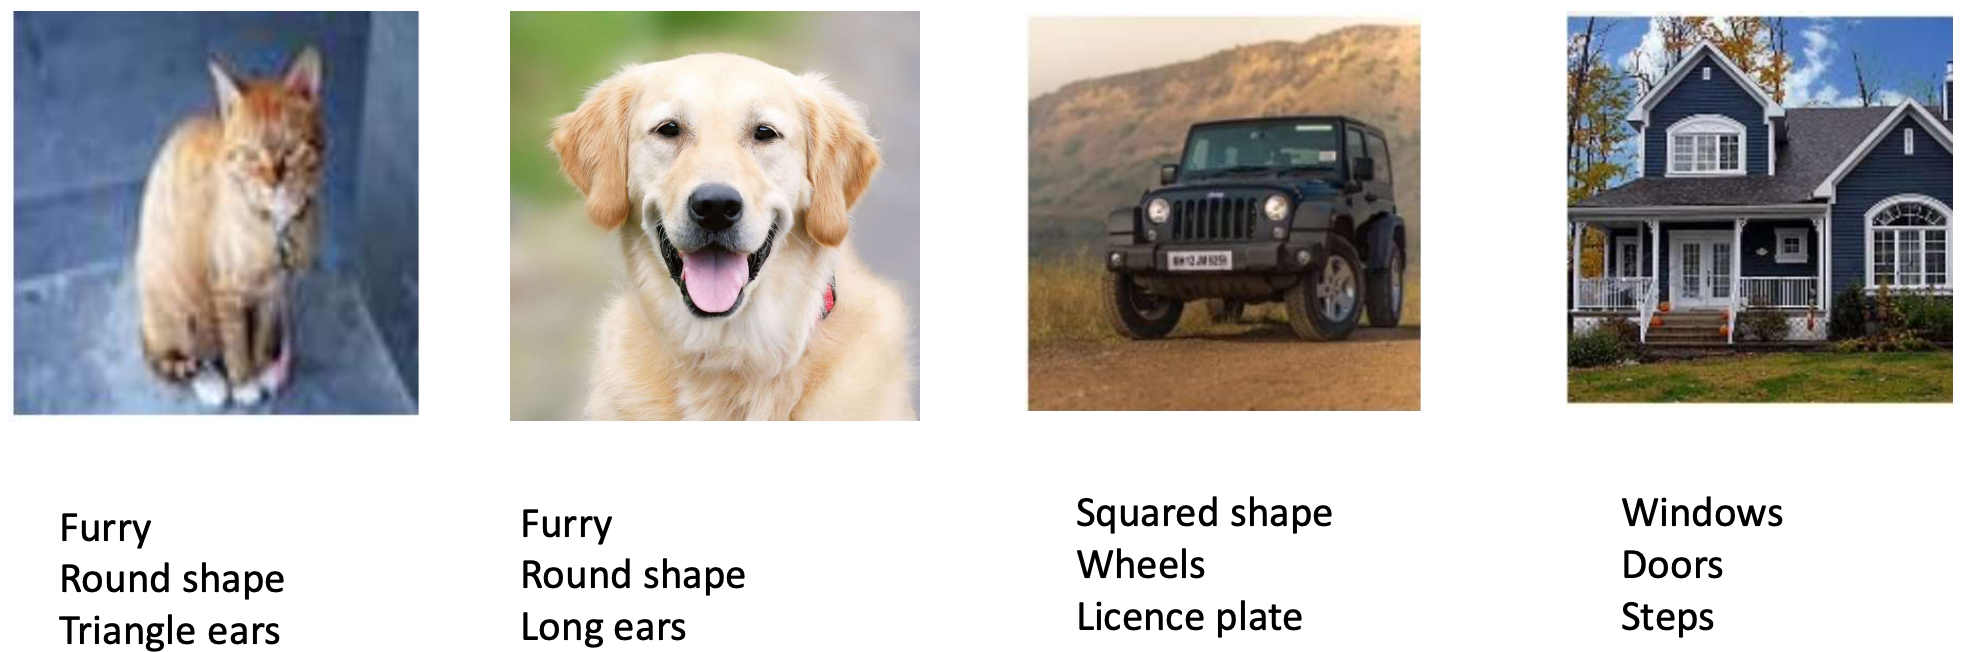
\includegraphics[scale=.5]{images/cnn/cv_problems.png}
    \centering
\end{figure}



Anche se le abbiamo rappresentate così, normalmente le features che le CNN imparano non possono essere descritte in termini così chiari.

\section{Perchè usare le CNN?}
Ci sono diverse motivazioni per cui le CNN sono una buona scelta. Uno di questi è che le reti neurali tradizionali non scalano bene per dati in forma di immagine mentre le \textbf{CNN sono specificamente pensate per image recognition task}.


I punti più forti delle CNN sono:
\begin{itemize}
    \item connesioni locali;
    \item condivisione dei pesi;
    \item pooling;
    \item gerarchia delle feature.
\end{itemize}
Passare attraverso tutte queste fasi (quali fasi?) è necessario a causa del fatto che non è possibile passare da pixels \textit{grezzi} (raw) a concetti astratti (es. \textit{MAN}). L'insieme di immagini per cui \textit{MAN} potrebbe essere appropriato crea una \textbf{regione molto contorta}. In questo contesto, passare attraverso diversi strati di astrazioni o feature è una buona strategia. Il \textbf{focus delle deep neural networks è andare attraverso tutti questi livelli di astrazione}.
\subsection{Gerarchia delle features}
\begin{figure}[!h]
    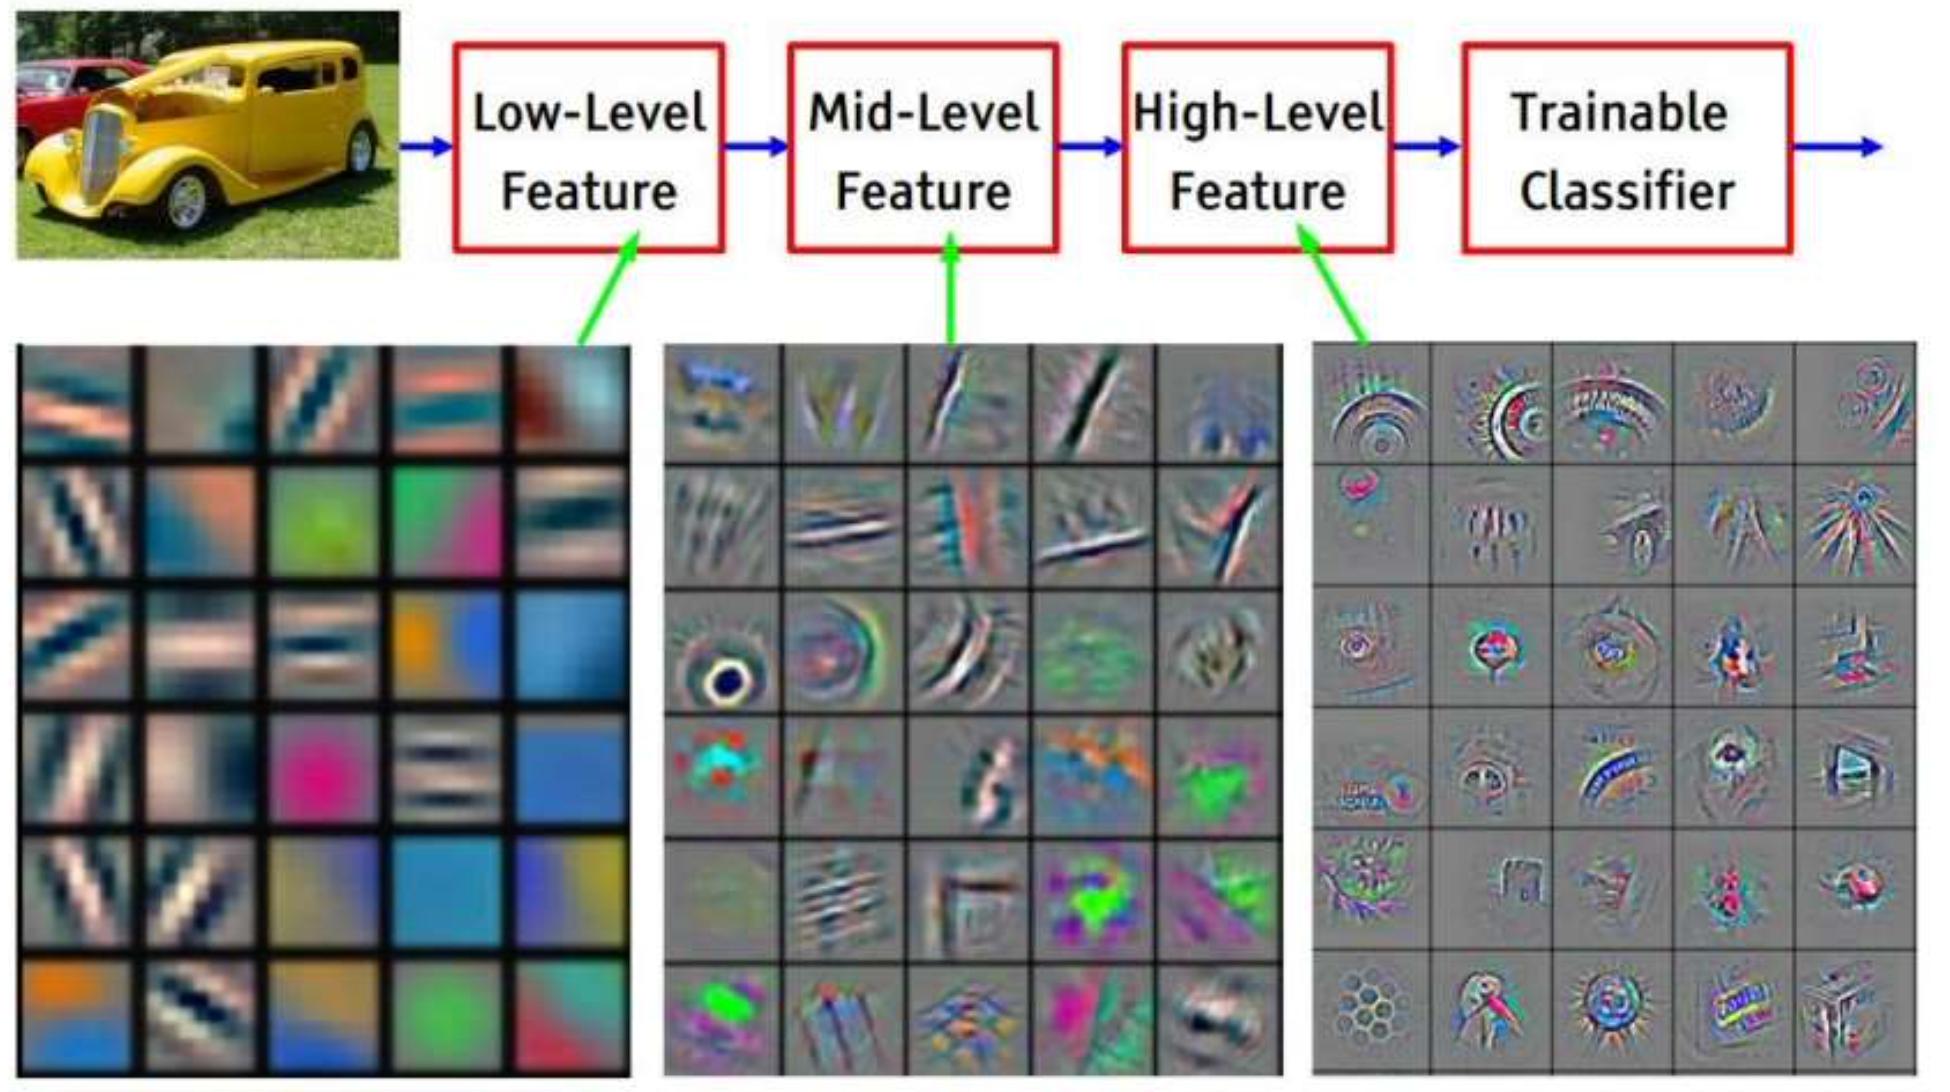
\includegraphics[scale=.45]{images/cnn/features_hierarchy01.png}
    \caption{Visualizzazione delle feature di una CNN trainata su ImageNet}
    \centering
\end{figure}


i livelli hanno crescenti livelli di astrazione e complessità crescente.



Queste sono le feature che massimizzano l'attivazione dei neuroni ad un dato livello.
\begin{figure}[!h]
    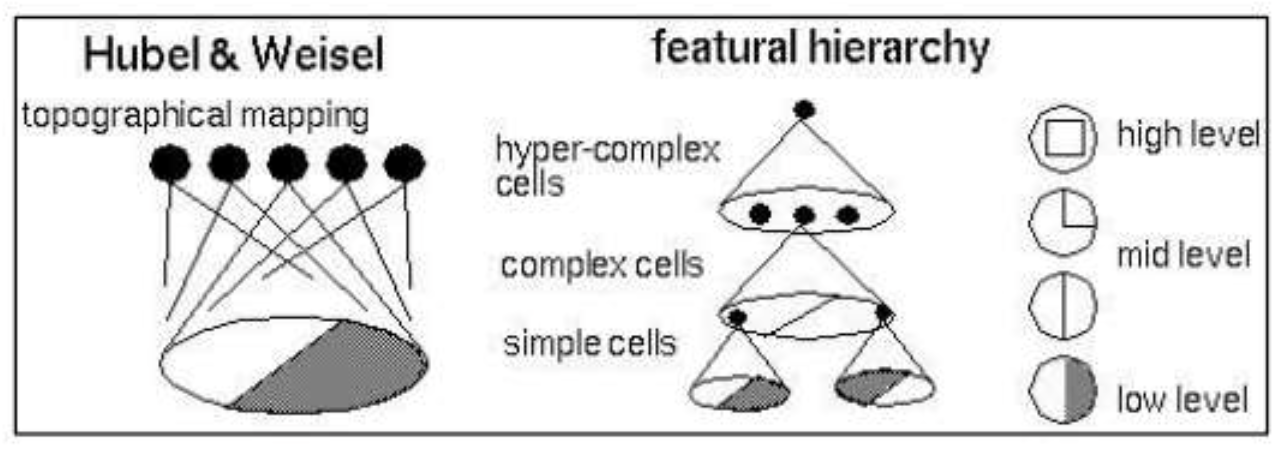
\includegraphics[scale=.5]{images/cnn/features_hierarchy02.png}
    \centering
\end{figure}
\newpage
IL multilayer perceptron non scala bene con immagini di grandi dimensioni.
\begin{figure}[!h]
    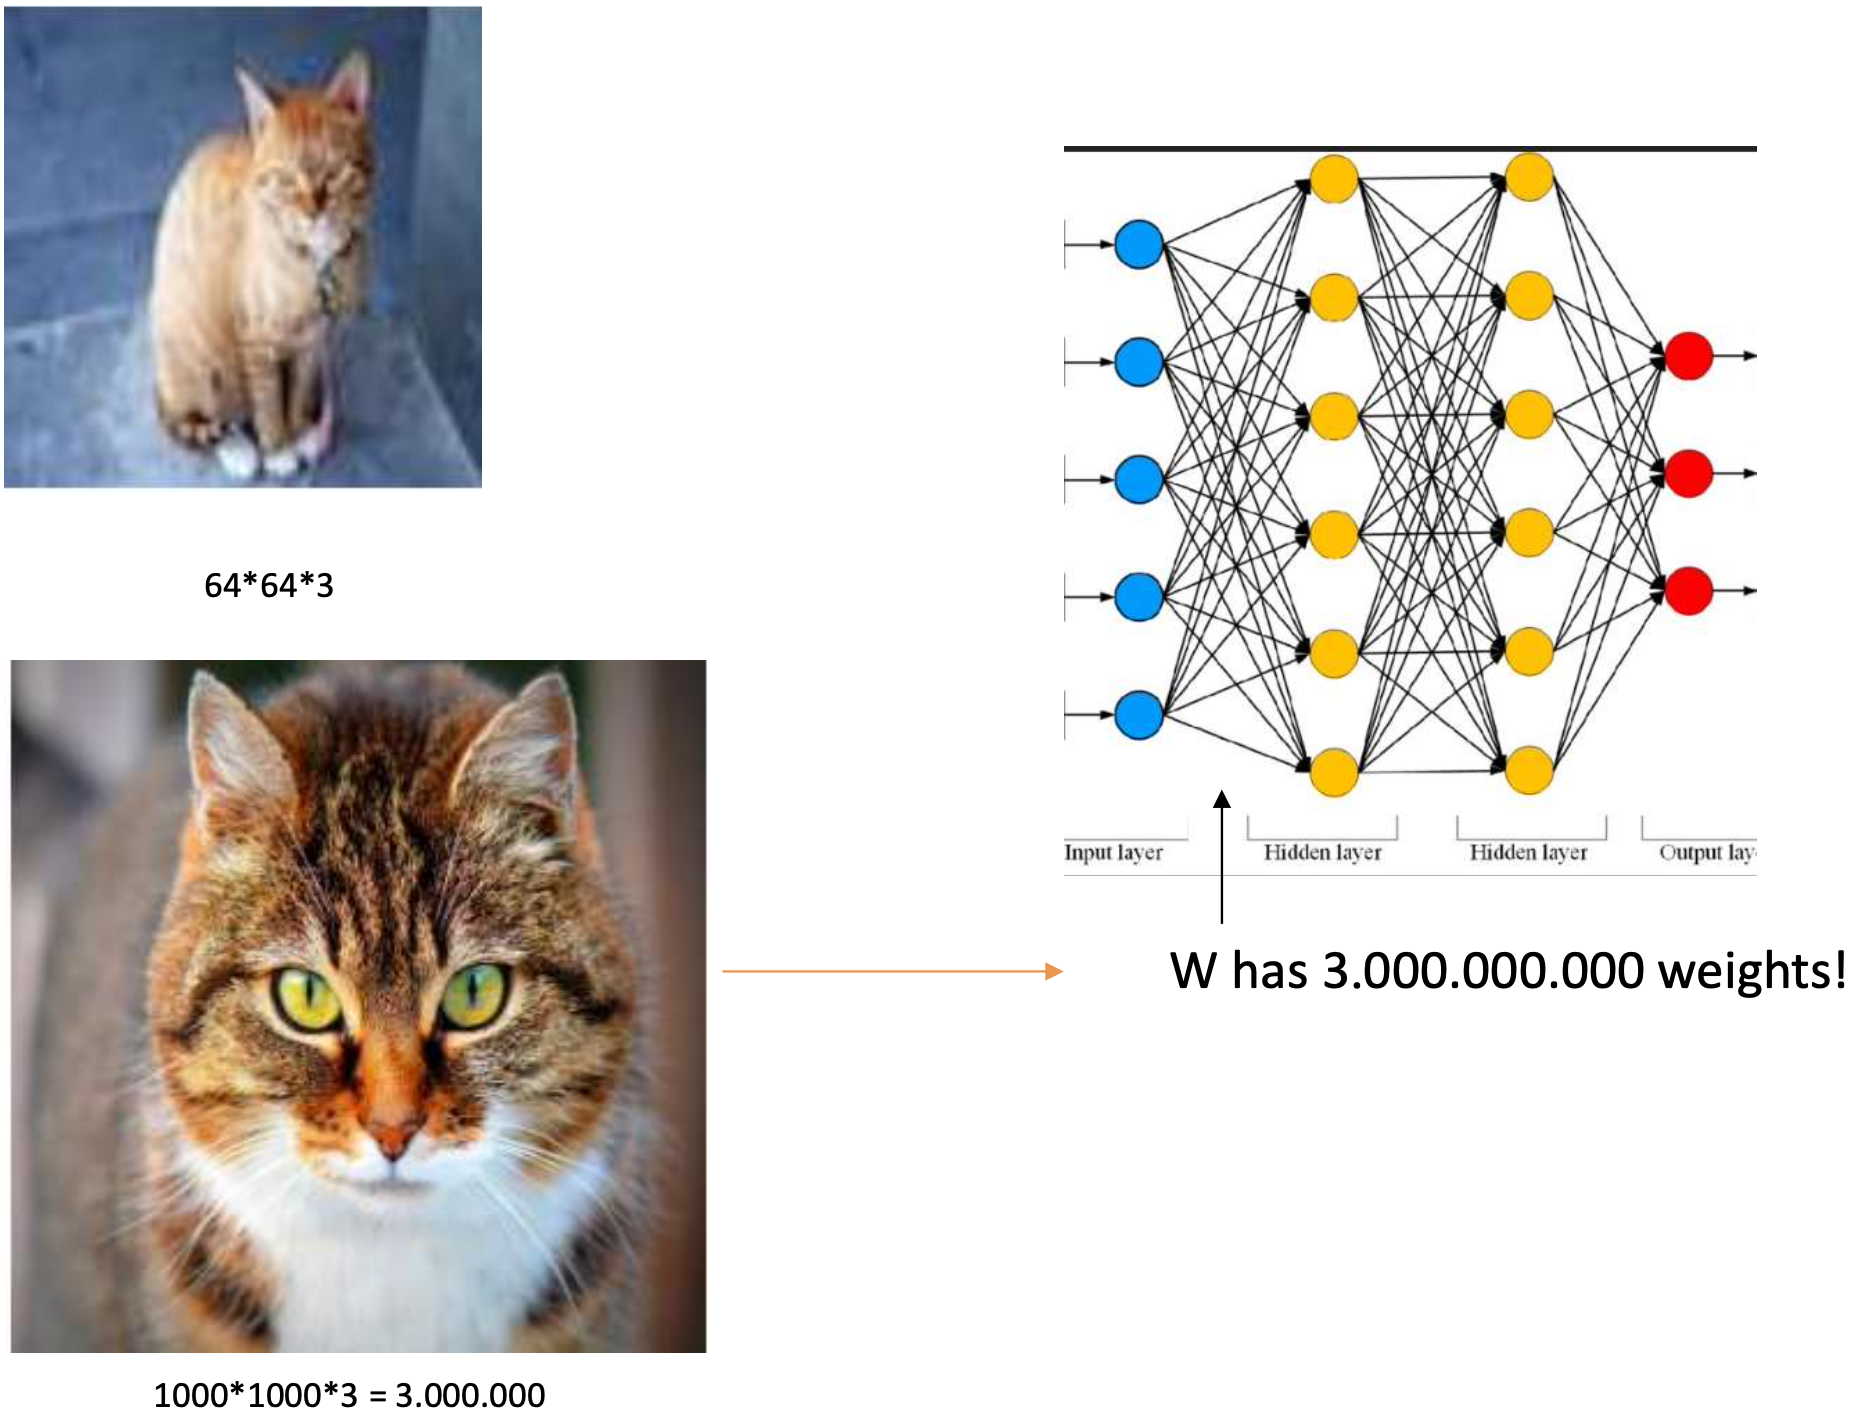
\includegraphics[scale=.5]{images/cnn/features_hierarchy03.png}
    \centering
\end{figure}



Inoltre, il multilayer perceptron perde l'informazione spaziale associata all'immagine.
\begin{figure}[!h]
    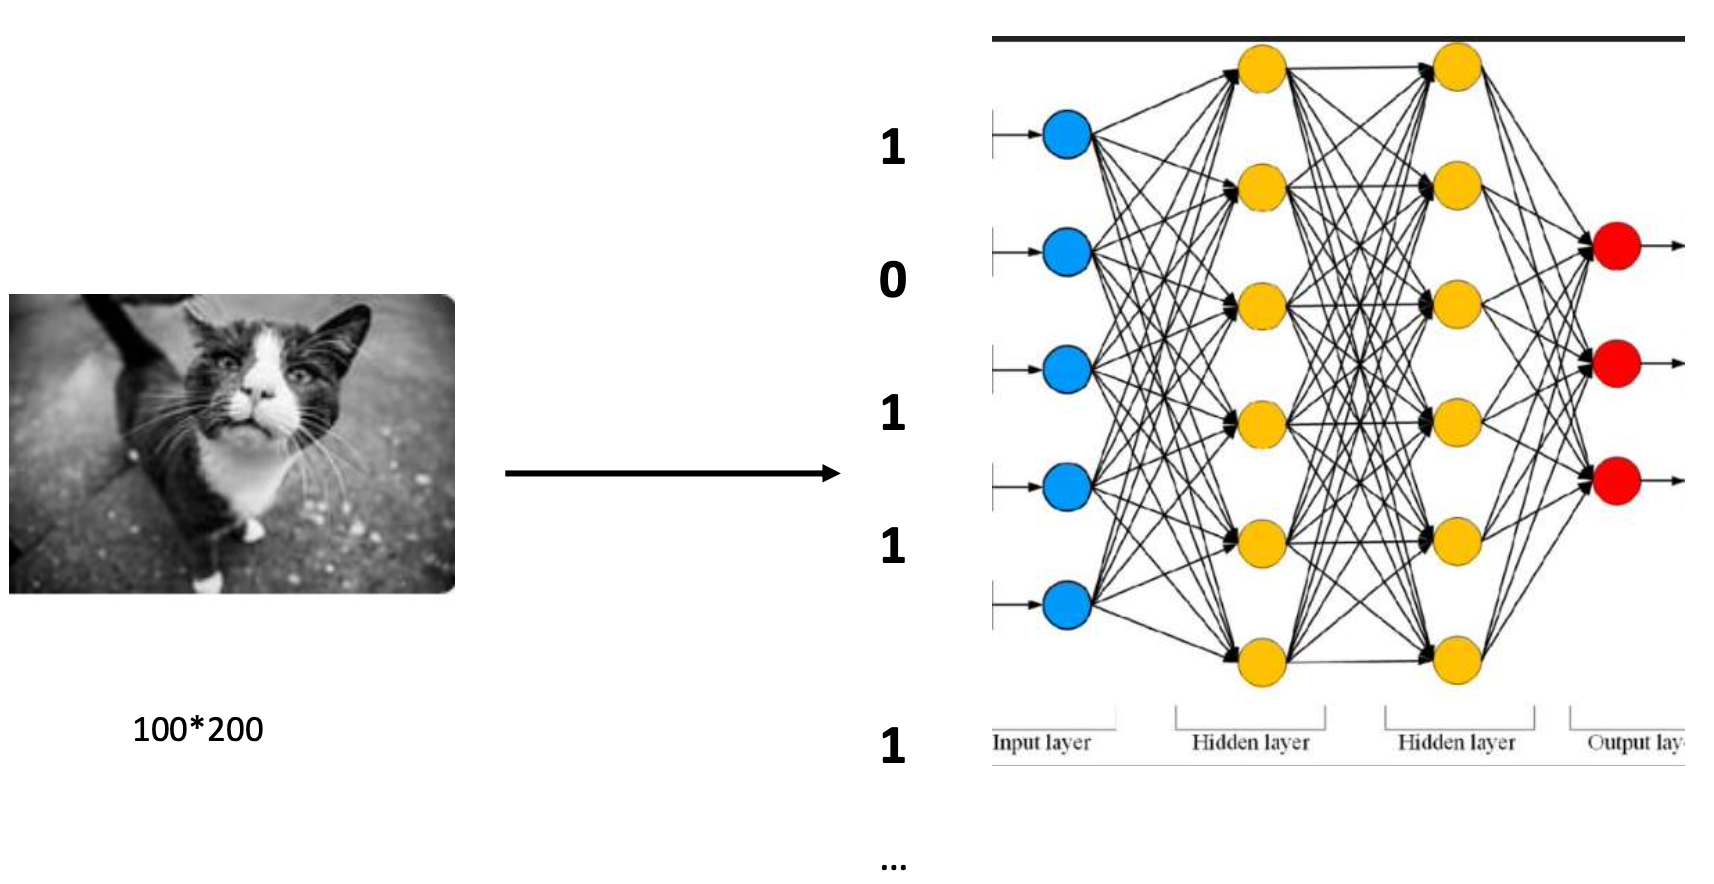
\includegraphics[scale=.5]{images/cnn/features_hierarchy04.png}
    \centering
\end{figure}
\newpage
\section{Architettura}
\begin{figure}[!h]
    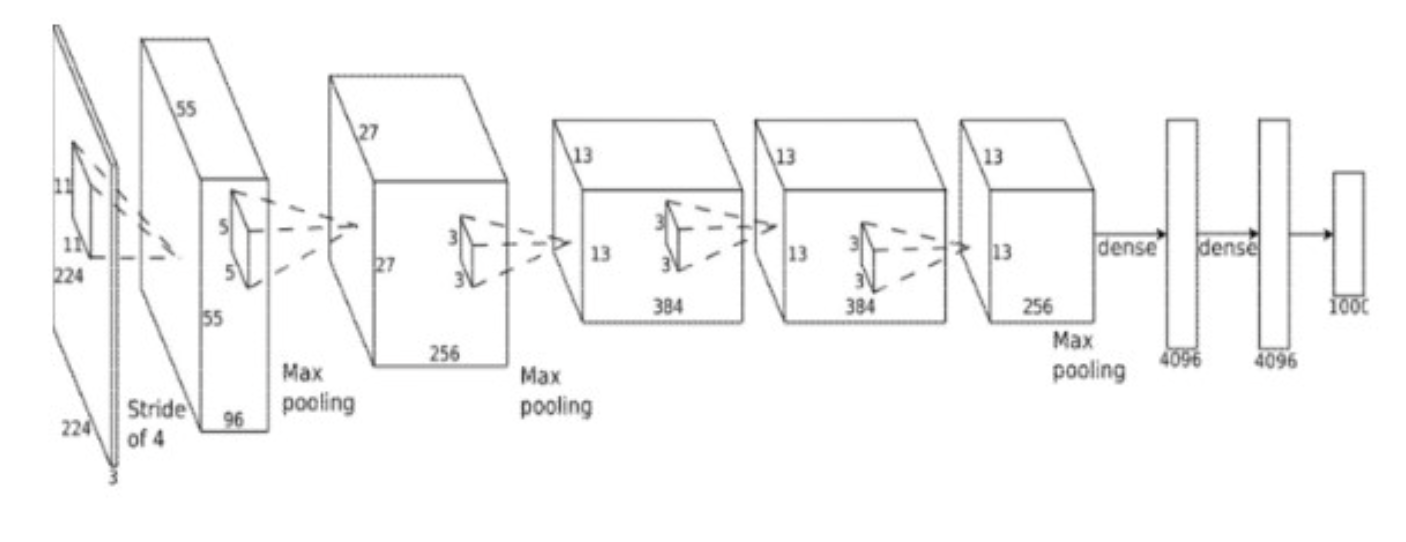
\includegraphics[scale=.5]{images/cnn/arch01.png}
    \centering
\end{figure}



Diversi layer, deep architecture, sono convolutional o max pooling e acrivation function nell'ultimo fully connected.questa è una tipica architettura delle conv net.


Gli \textbf{elementi base} di una CNN sono i seguenti
\begin{figure}[!h]
    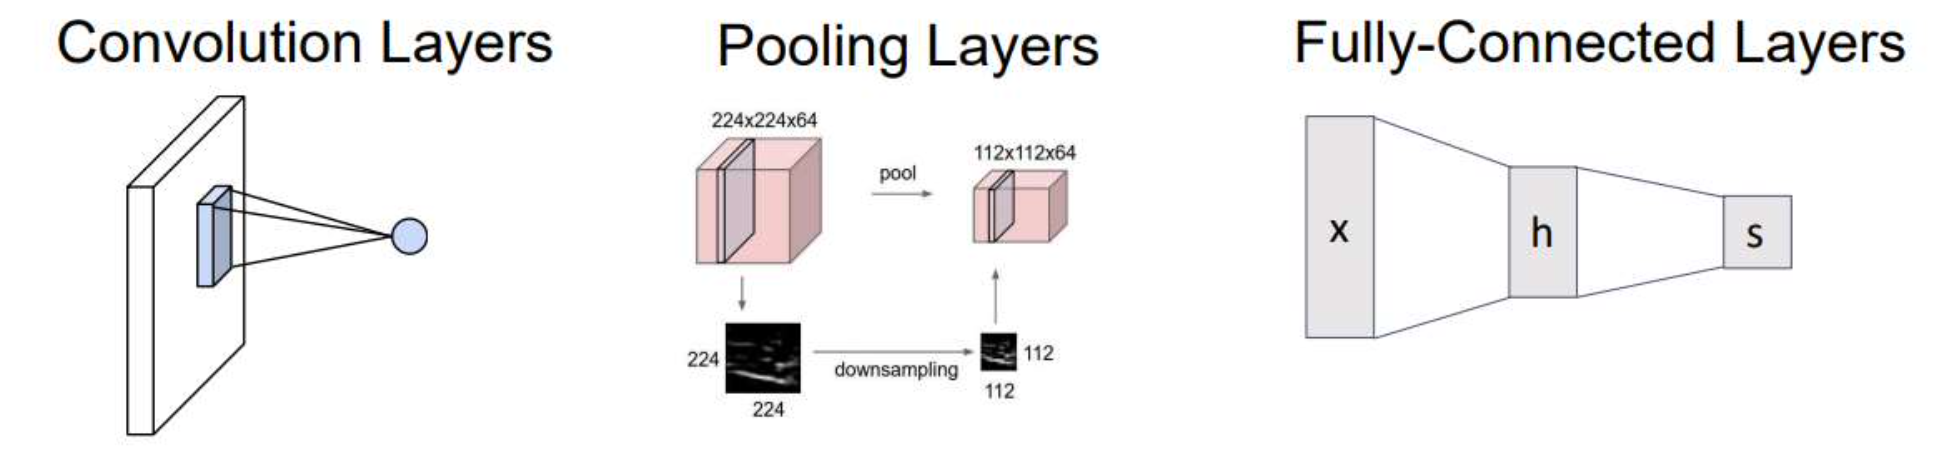
\includegraphics[scale=.45]{images/cnn/arch02.png}
    \centering
\end{figure}


Con la seguente \textbf{funzione di attivazione}
\begin{figure}[!h]
    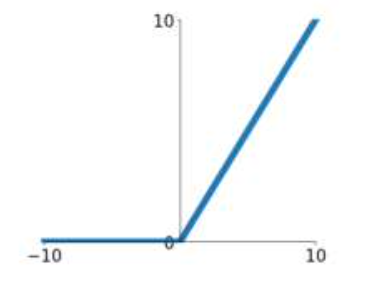
\includegraphics[scale=1]{images/cnn/act_fun.png}
    \centering
\end{figure}
\newpage
\subsection{Convolutional Layers}
Invece di \textbf{linearizzare l'immagine} e perdere informazione spaziale, le hidden units sono connesse ad una porzione (\textbf{patch}) dell'immagine: il \textbf{campo recettivo dell'unità}.
\begin{figure}[!h]
    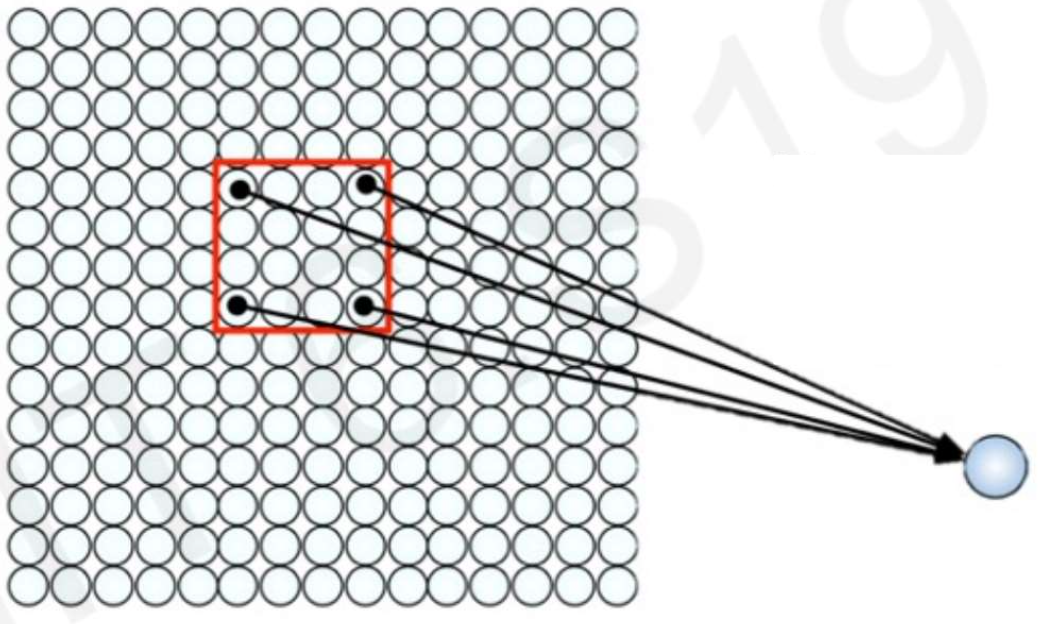
\includegraphics[scale=.5]{images/cnn/conv_layer.png}
    \centering
\end{figure}



Questa unità vede solo una piccola regione dell'immagine. Il vettore dei pesi è detto \textbf{filtro}, o \textbf{kennel}, e determina il tipo di feature per le quali l'unità si deve attivare in maniera maggiore.



L'unità di attivazione è
\begin{equation}
    z=ReLU(w^Tx+w_0),
\end{equation}
con $w$ e $x$ che sono le \textbf{rappresentazioni vettoriali} dei valori e dei pesi dei pixel. Il bias è invece rappresentato da $w_0$. 
\begin{figure}[!h]
    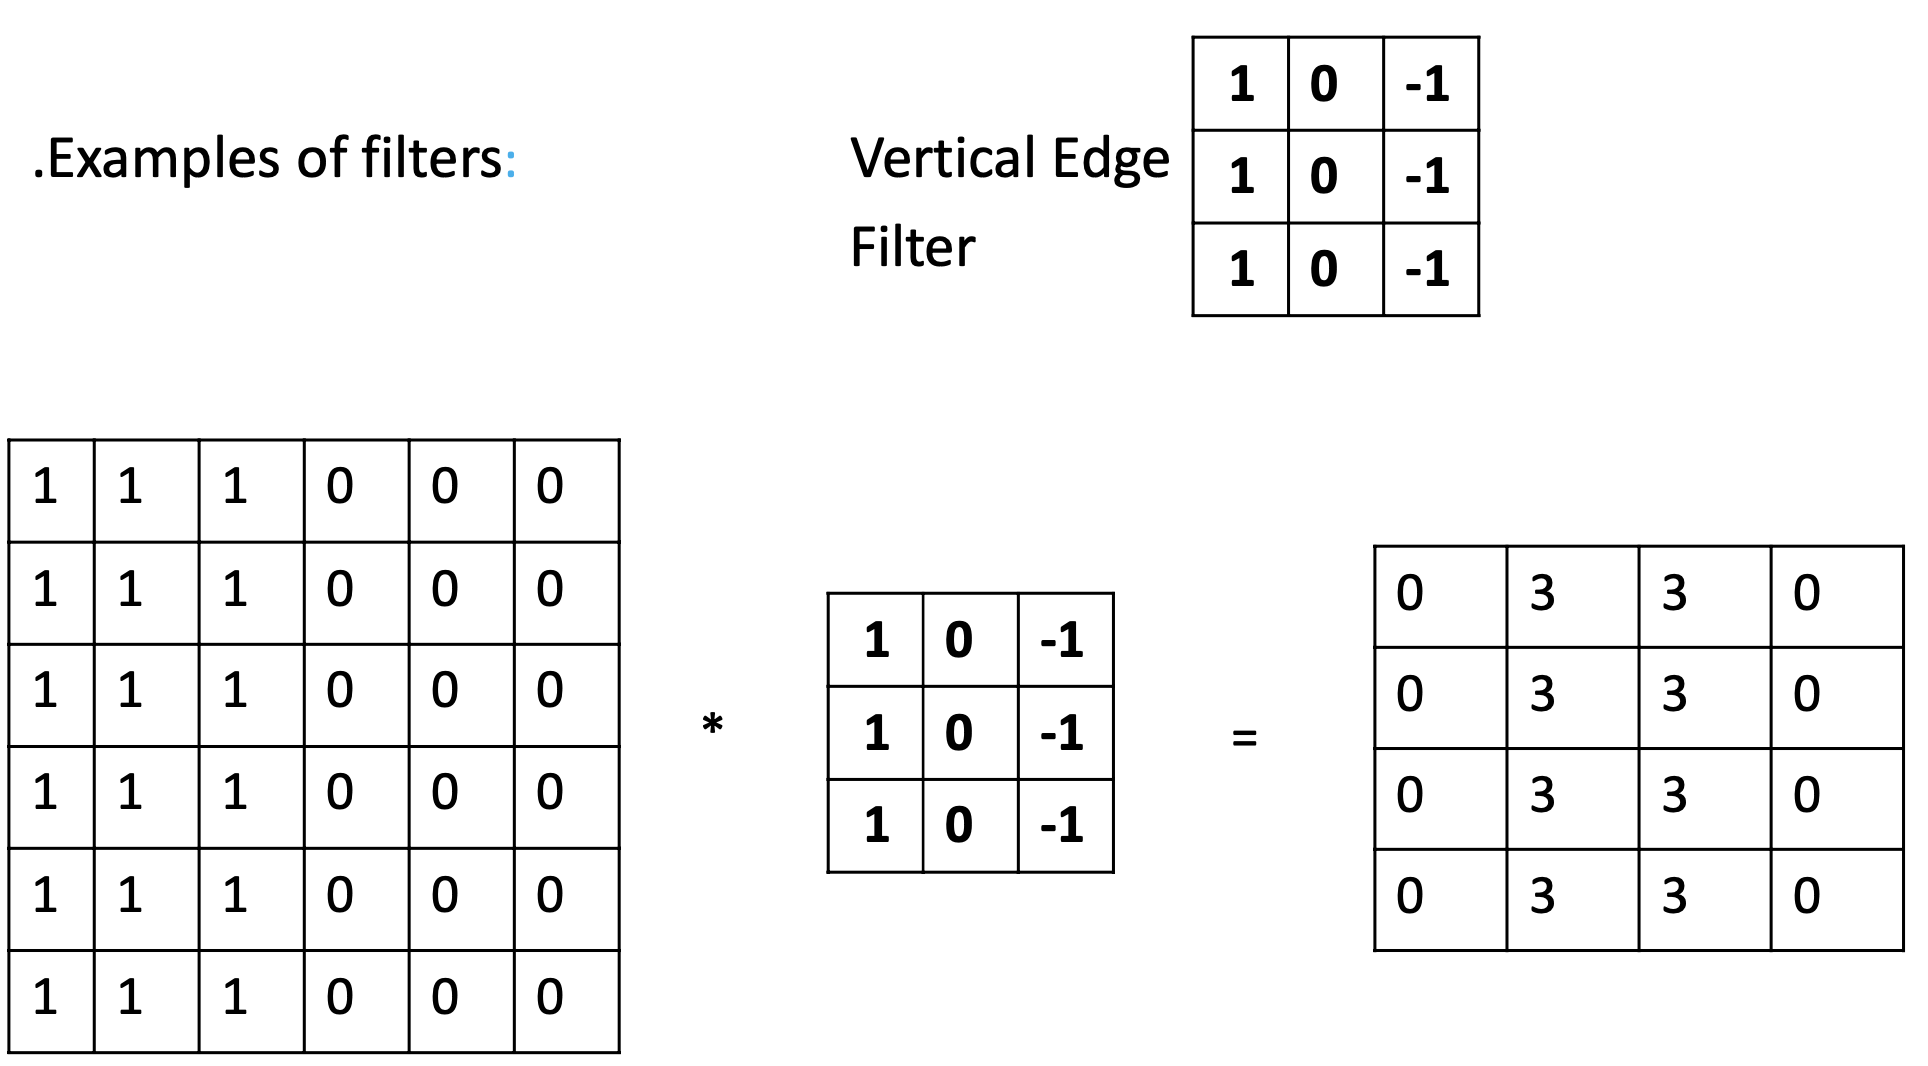
\includegraphics[scale=.5]{images/cnn/filter_ex.png}
    \centering
\end{figure}
\newpage
\subsubsection{Feature Maps}
Diverse unità di un hidden layer formano uno \textbf{feature map}.
\begin{figure}[!h]
    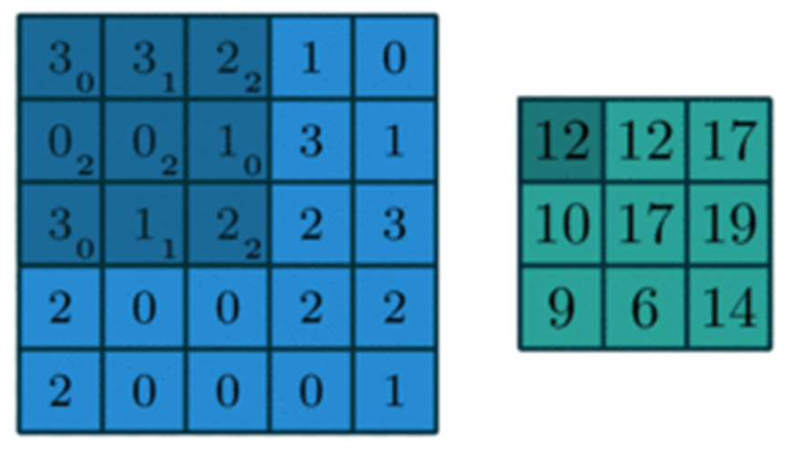
\includegraphics[scale=.5]{images/cnn/feature_maps.png}
    \centering
\end{figure}


I \textbf{convolutional layers contengono un insieme di feature mpas, ognuna con un filtro diverso}.
\newline
\newline
Altri esempi di filtri convoluzionali sono i seguenti
\begin{figure}[!h]
    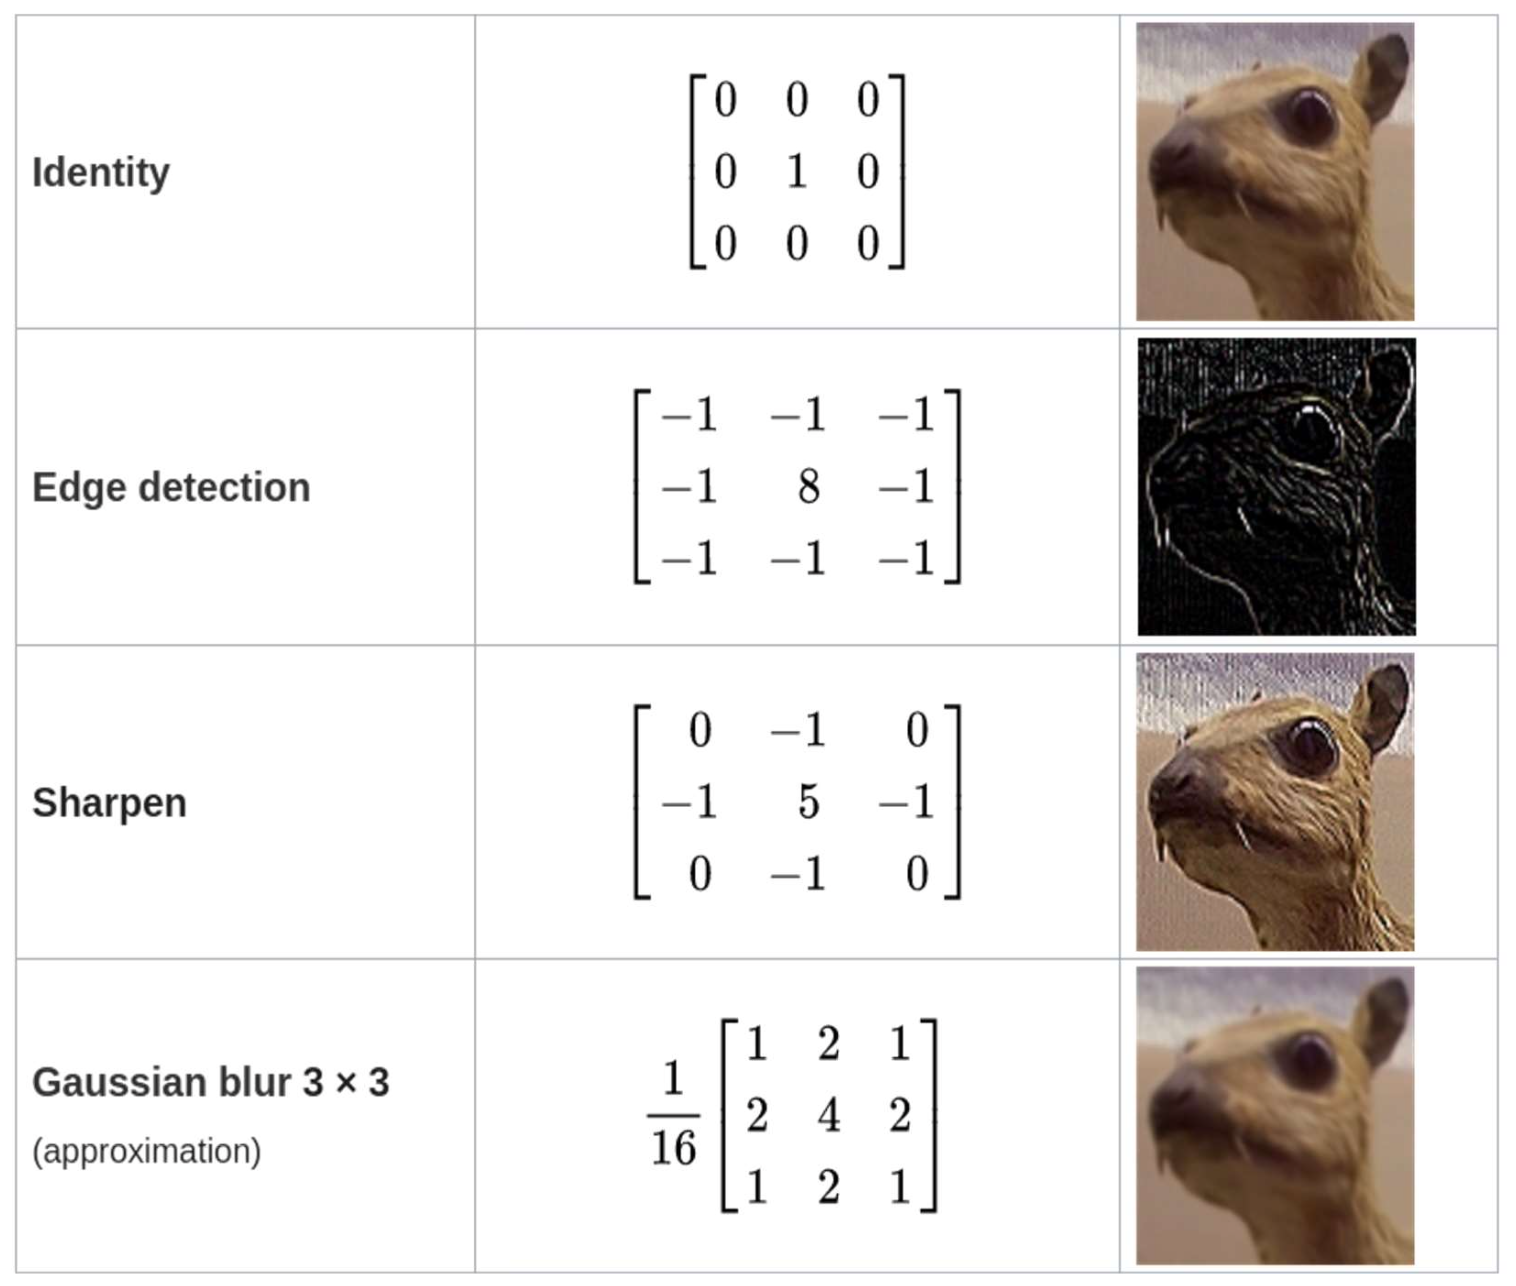
\includegraphics[scale=.7]{images/cnn/conv_filter_ex.png}
    \centering
\end{figure}
\newpage
\subsubsection{Proprietà}
Le proprietà principali dei convolutional layer sono:
\begin{itemize}
    \item sparsità dei pesi;
    \item condivisione dei (pesi dei) parametri;
    \item analisi basata sulla località;
    \item \textbf{equivalenza alla traduzione}, se una feature (diciamo un occhio) viene individuata in una posizione, potrebbe essere individuata anche in un'altra posizione mai vista prima per mezzo dello stesso filtro. Ciò attiverebbe una unità nello stesso layer ma possibilmente in una location differente.
\end{itemize}
\subsubsection{Translation Equivariance}
\begin{itemize}
    \item a basso livello (feature extraction): lo stesso filtro rileva la stessa feature (ad esempio un bordo o un occhio) anche se in una posizione diversa. Ciò attiverà un'unità vicina nella stessa feature map;
    \item a livello di classificazione: ad un particolare oggetto dovrebbe essere assegnata la stessa classificazione indipendentemente dalla sua posizione all'interno dell'immagine (ottenibile con piccole traduzioni o comunque con data augmentation).
\end{itemize}
\begin{figure}[!h]
    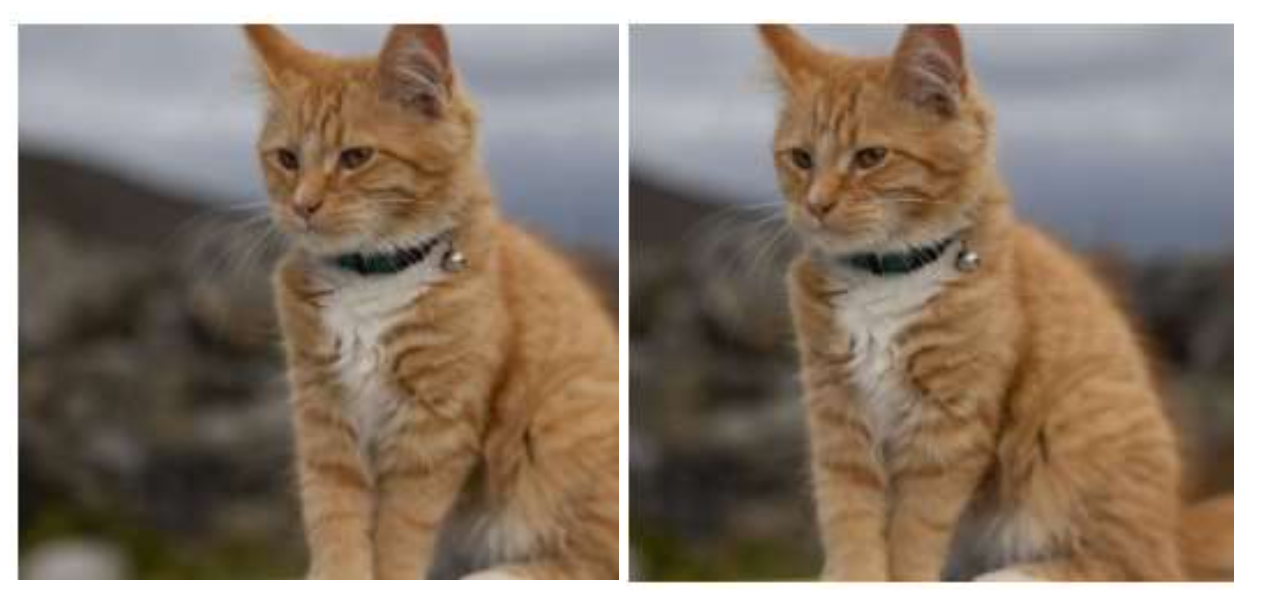
\includegraphics[scale=.5]{images/cnn/trans_inv.png}
    \centering
\end{figure}
\newpage
\subsubsection{Iperparametri}
Sono fissi in base all'architettura. Cambiano di architettura in architettura.
\begin{itemize}
    \item \textbf{kernel size}, normalmente è pari (es $3\cdot3$). Più è grande il kernel, più è piccola la feature map;
        \begin{figure}[!h]
            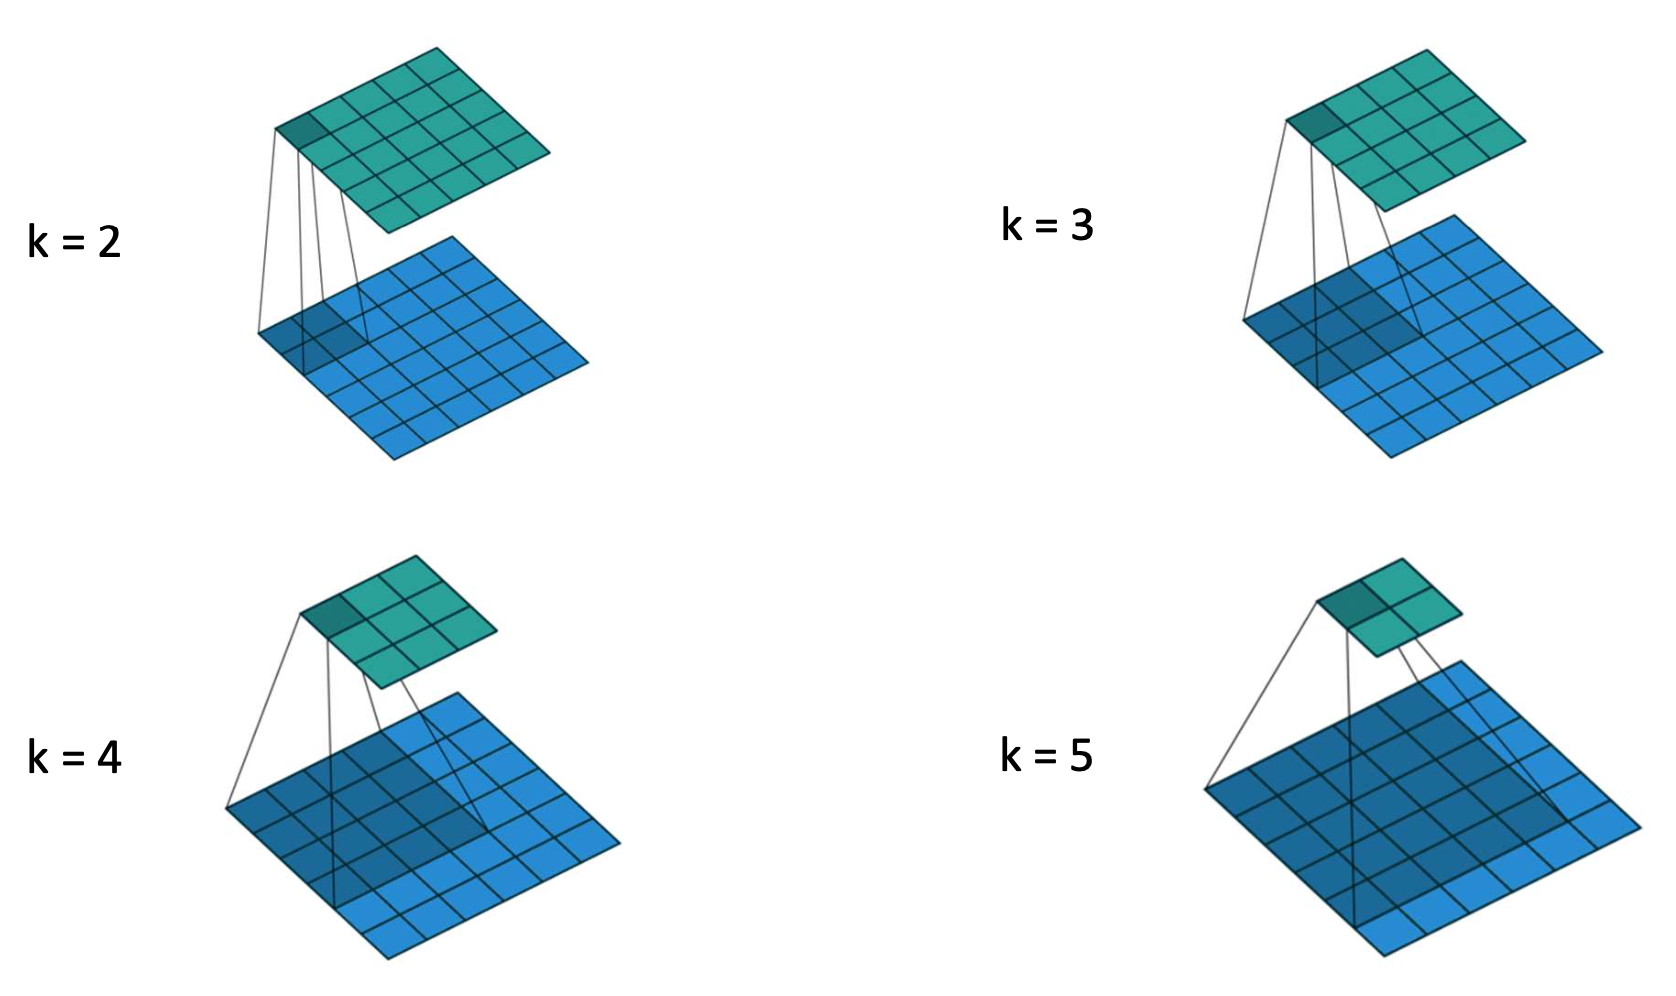
\includegraphics[scale=.25]{images/cnn/kernel_size.png}
            \centering
        \end{figure}
    \item \textbf{passo uno}, il filtro viene spostato un pixel alla volta, $S$ viene spostato in passi più grandi di dimensione $S$ ($S$ = passo). Di nuovo, più grande è il passo, più piccola è la feature map;
        \begin{figure}[!h]
            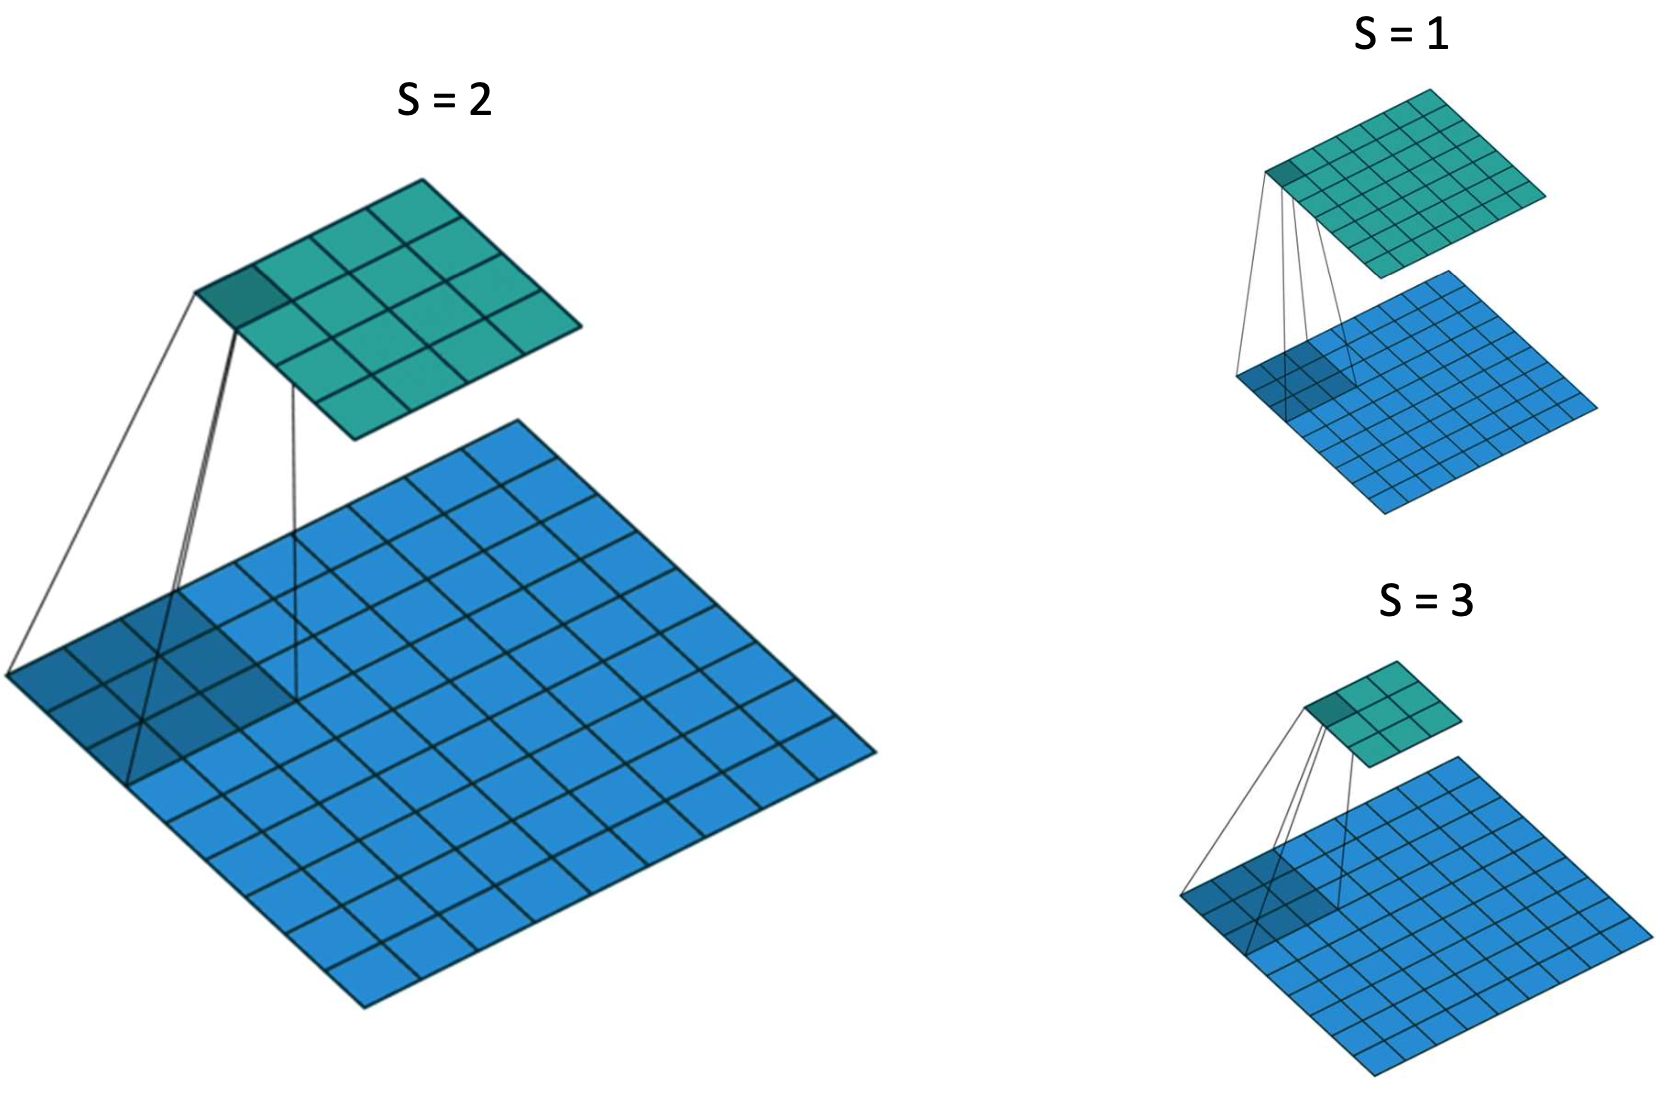
\includegraphics[scale=.25]{images/cnn/stride.png}
            \centering
        \end{figure}
    \item \textbf{padding}, l'immagine originale con pixel aggiuntivi attorno all'esterno (così che la feature map possa avere le stesse dimensioni dell'immagine originale);
        \begin{figure}[!h]
            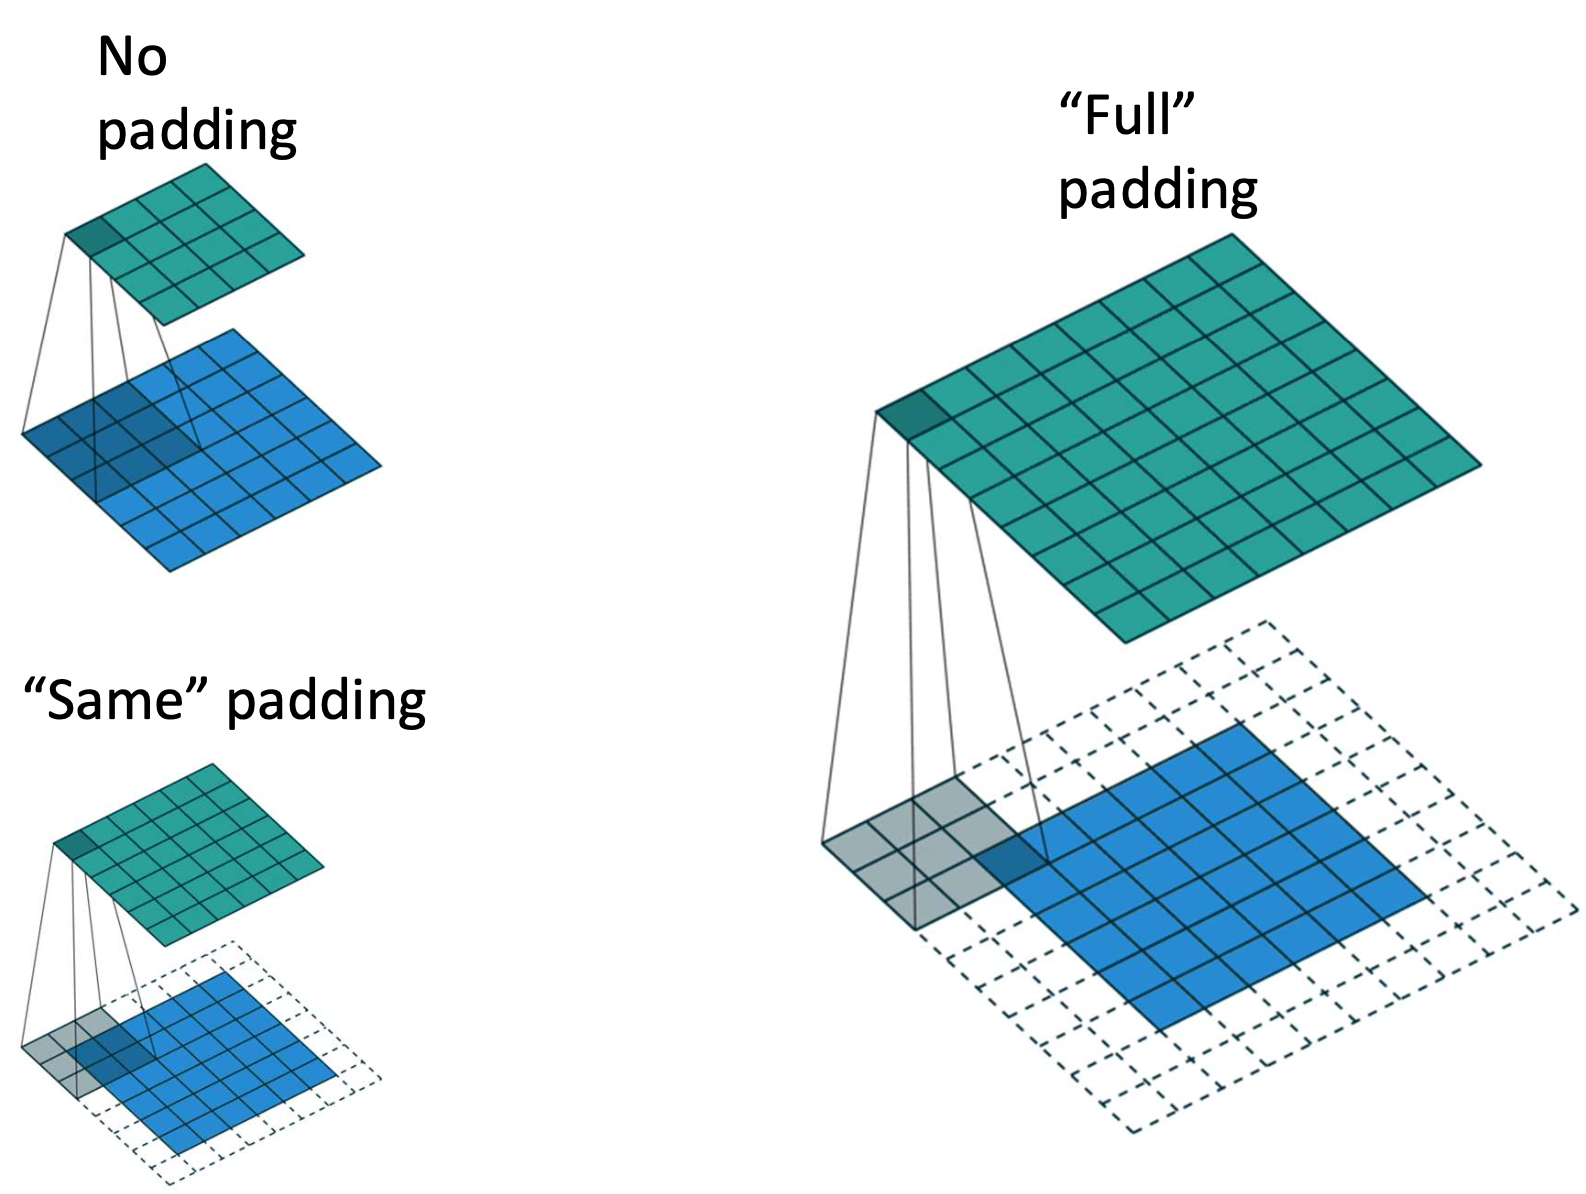
\includegraphics[scale=.25]{images/cnn/padding.png}
            \centering
        \end{figure}
    \item \textbf{il numero di filtri convoluzionali}, delle feature maps nei convolutional layer.
\end{itemize}
\newpage
\subsubsection{Filtri}
Nell'elaborazione classica delle immagini, il peso dei kernel veniva \textbf{fatto a mano} da esperti.
Le reti neurali convoluzionali, invece, \textbf{imparno} i pesi migliori (utilizzando l'algoritmo di backpropagation).
I reali filtri appresi sono ovviamente molto meno chiari e interpretabili rispetto agli esempi che abbiamo realizzato noi. 
\begin{figure}[!h]
    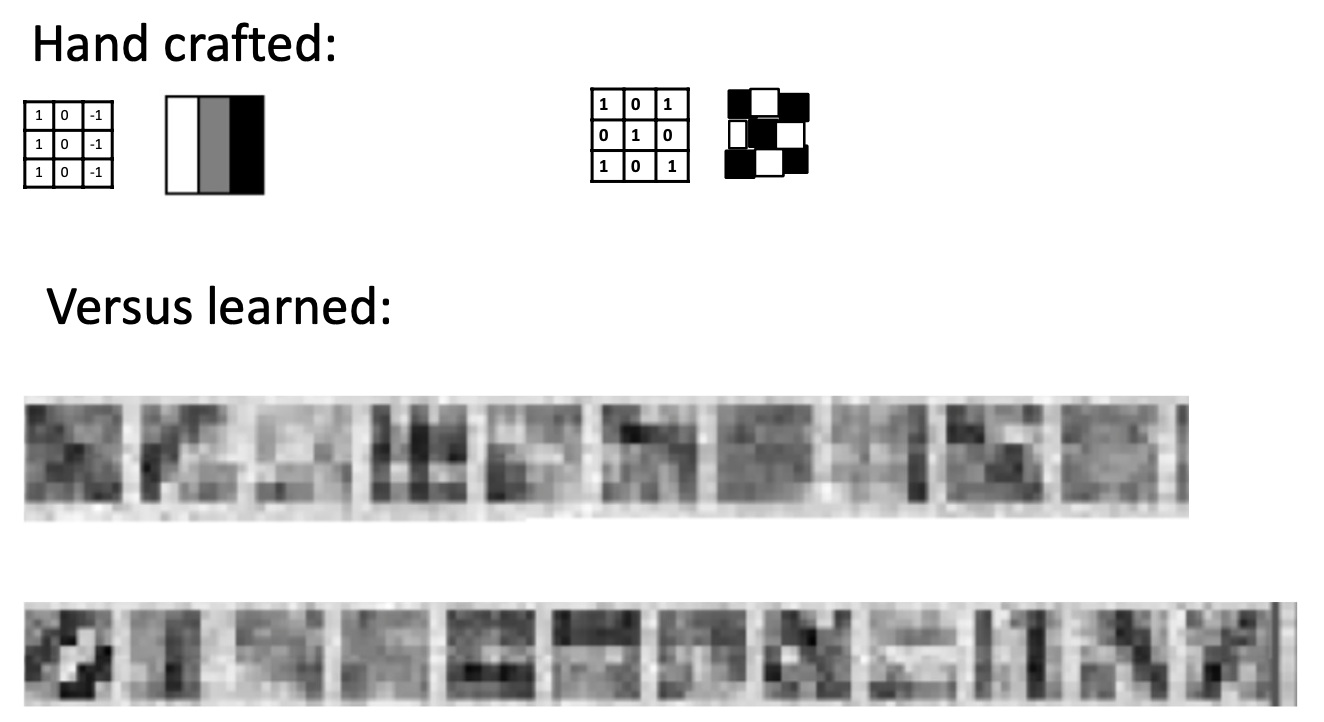
\includegraphics[scale=.7]{images/cnn/filters.png}
    \centering
\end{figure}
\newpage
\section{Multidimensional Convolution}
\paragraph{Input level.}
L'immagine mostra un filtro multi dimensionale che accetta inputt attravero i canali \textbf{R}, \textbf{B} e \textbf{B}. Questo kernel in particolare ha $27$ pesi ($9\cdot 3$) (più un parametro bias che non è esplicitato) e può essere visualizzato come un tensore $3\times3\times3$ con $3$ calari rappresentabili con diversi colori.
\begin{figure}[!h]
    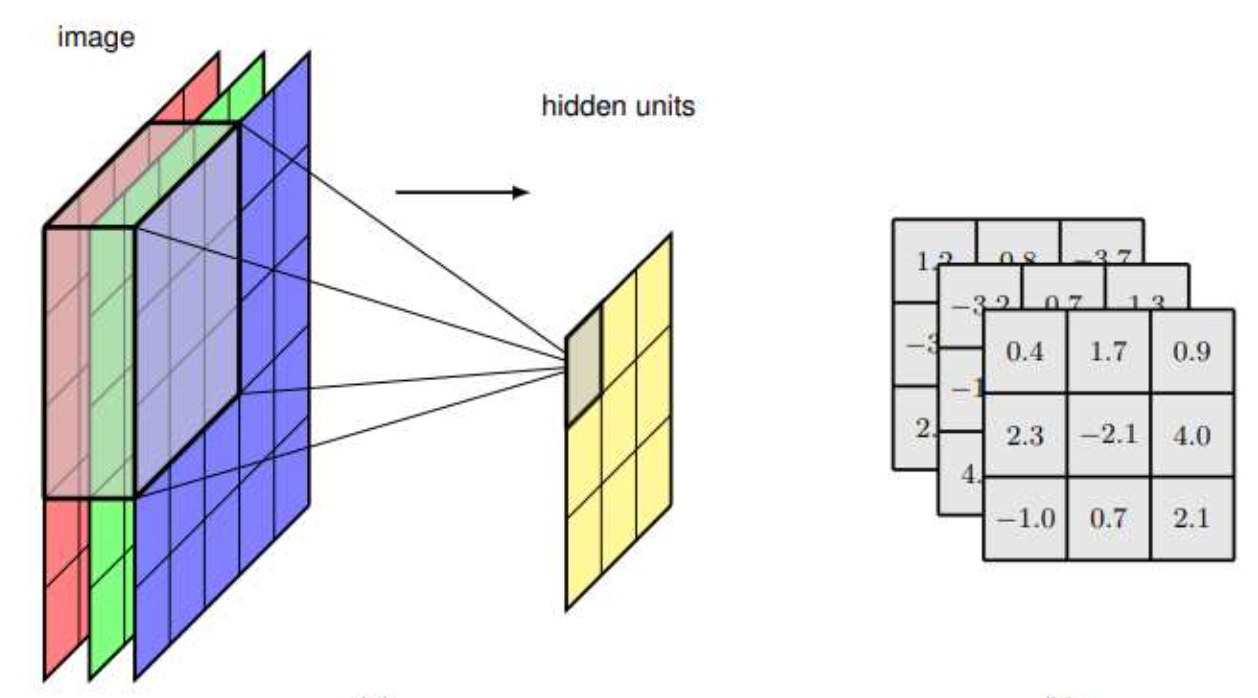
\includegraphics[scale=.35]{images/cnn/multid_conv.png}
    \centering
\end{figure}



\textbf{Nota:} quanto detto vale per il primo livello del kernel. Per livelli più alti il numero di canali di ingresso è in generale maggiore di 3 quindi i filtri non sono rappresentati direttamente.


\paragraph{Visualizzare i filtri (first convolutional layer).} Segue un esempio di un altro filtro estrato dal first convolutional layer di \textbf{AlexNet}.
\begin{figure}[!h]
    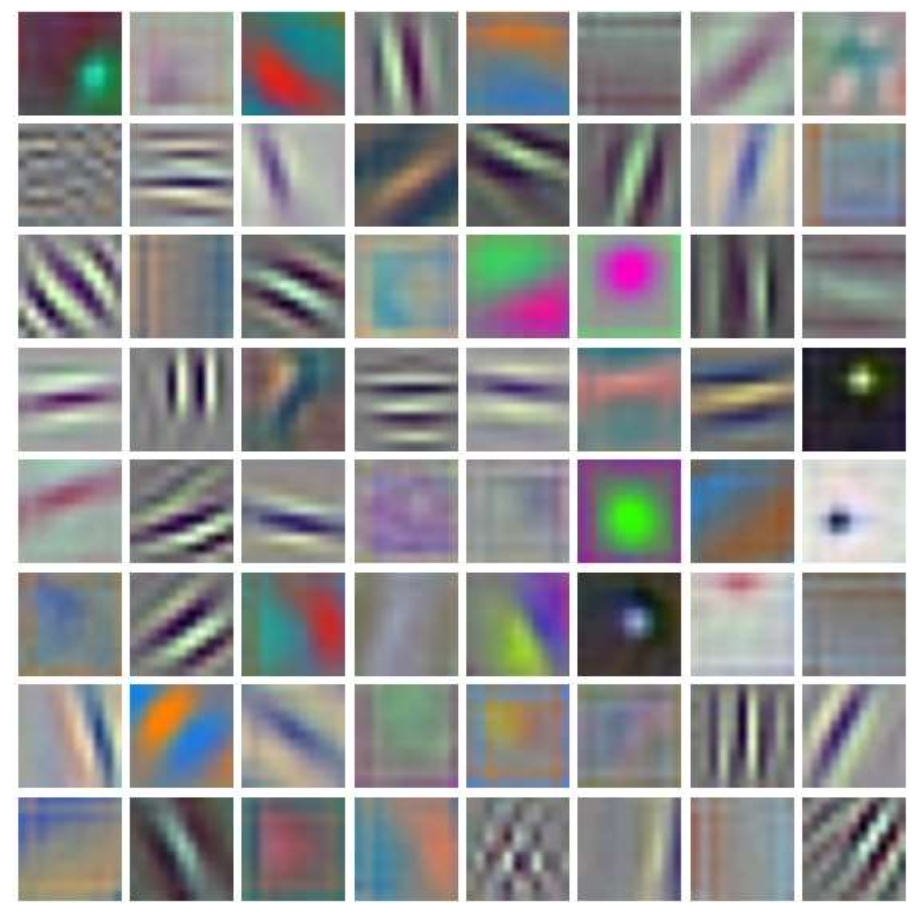
\includegraphics[scale=.3]{images/cnn/alexnet.png}
    \centering
\end{figure}



Uno dei problemi di queste reti è che \textbf{sono opache}, cioè \textbf{i filtri nei livelli più profondi non possono essere visualizzati direttamente} (in genere quando ci sono più di tre canali). Per i livelli più deep e lontani dall'input, \textbf{diventa quindi difficile capire quali feature hanno estratto ed imparato}. In letteratura esistono alcune tecniche che possono aiutarci: nel primo livello in realta, riusciamo a vedere il filtro applicato all'immagine. Quando però ci allontaniamo e arriviamo a kernel con profondità 32 o 64 (indicano il numero di canali analizzati alla volta), non si riesce più a vederli perchè non riusciamo a vedere immagini rgb. Un primo approccio alla risoluzione di questo problema consiste nella visualizzazione della patch di input che massimizza l'attivazione per tutti i neuroni di una determinata feature map.
\begin{figure}[!h]
    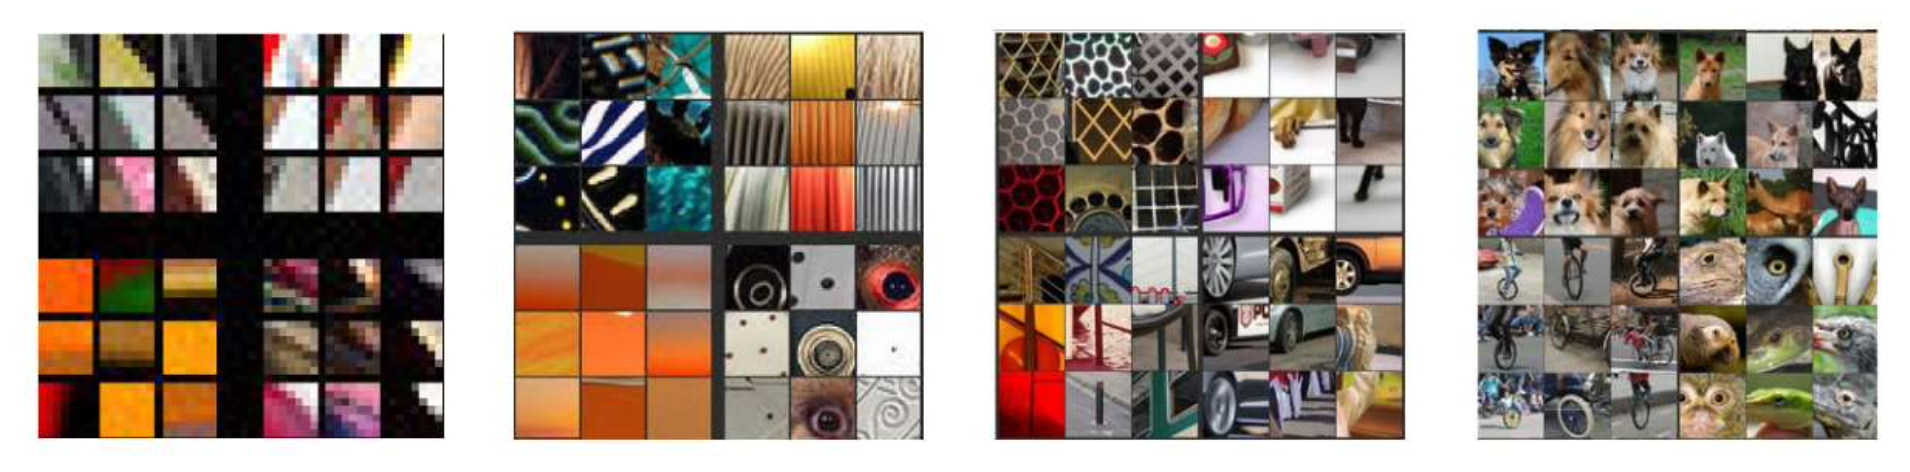
\includegraphics[scale=.3]{images/cnn/filters02.png}
    \centering
\end{figure}



Esempio di immagine che produce la maggiore attivazione nelle hidden units in una rete trainata su ImageNet. Le prime nove attivazioni in ciascuna feature map sono disposte in una griglia $3\times3$ per quattro canali scelti casualmente in ciascuno dei livelli corrispondenti. Si nota una progressione costante nella complessità al crescere della profondità, dai bordi semplici nel primo layer agli oggetti completi nell'ultimo layer.
\newpage
\paragraph{Altre tecniche di visualizzazione: saliency map.}
Le \textbf{saliency maps} possono essere utilizzate per identificare le regioni di un'immagine che sono più significative nel determinare l'etichetta della classe.
\begin{figure}[!h]
    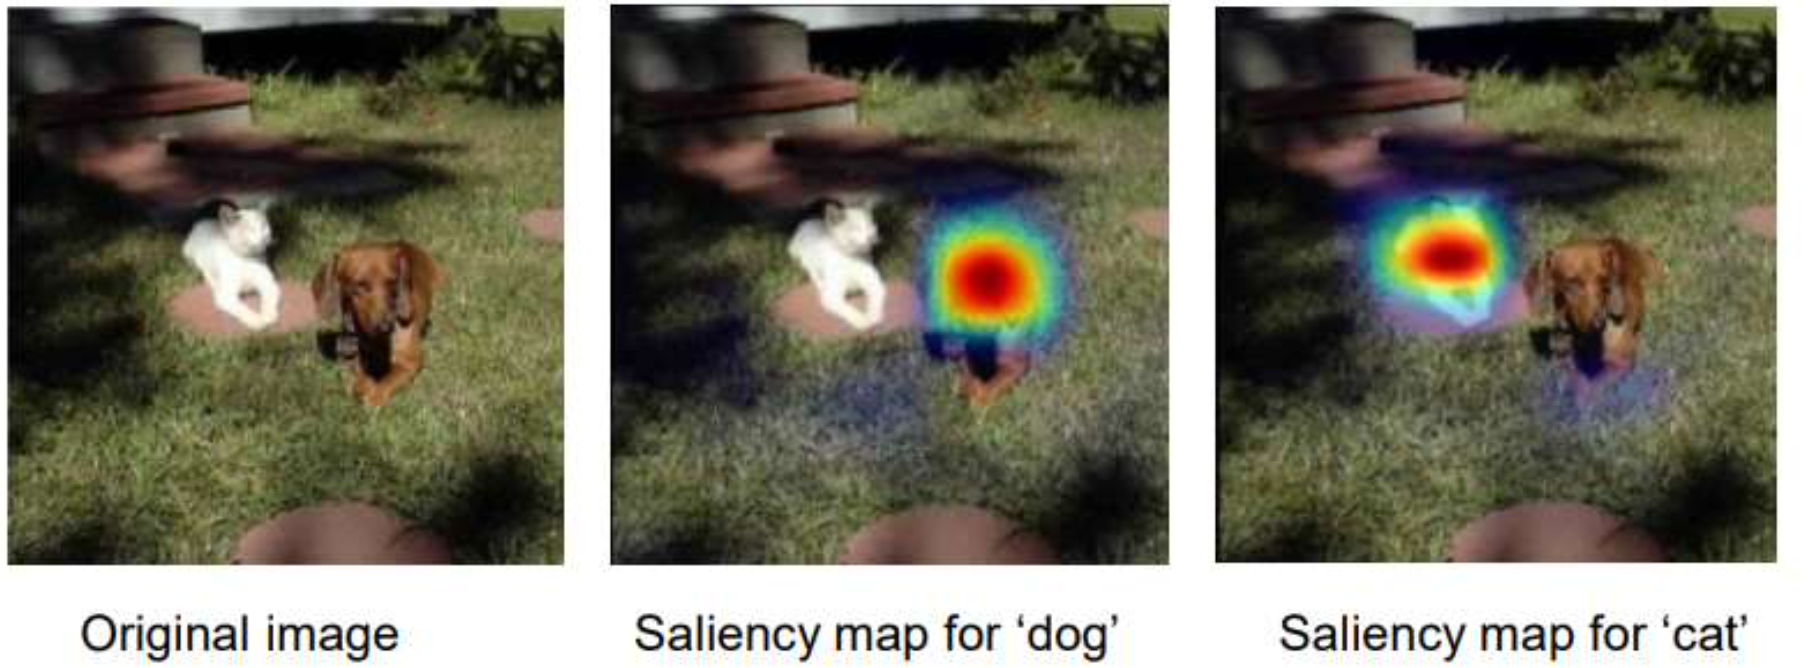
\includegraphics[scale=.4]{images/cnn/saliency_map.png}
    \centering
\end{figure}


\paragraph{Multidimensional convolution: multipli kernel indipendenti, multiple feature maps.} Multipli filtri (kernel) indipendenti portano a multple feature maps, andando a formare un unico \textbf{convolutional layer}.
\begin{figure}[!h]
    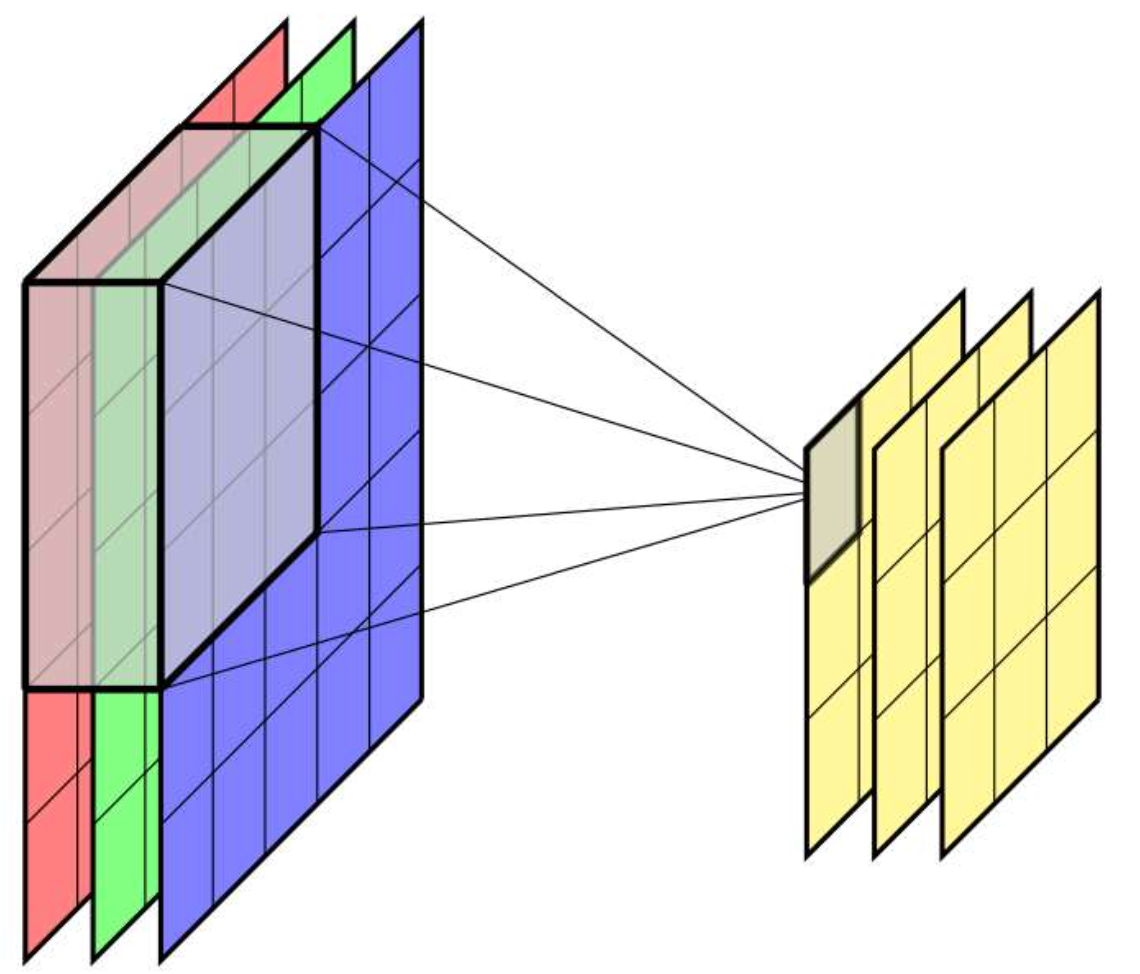
\includegraphics[scale=.3]{images/cnn/mult.png}
    \centering
\end{figure}


\paragraph{Multidimensional convolution : quanti pesi?} 
Il filtro opera su una porzione del volume in input. Nell'esempio, ogni neurone nel volume di output è connesso a $5\times5\times3=75$ neuroni del livello precedente.


Ogni fetta di neuroni (alla stessa profondità) denota una feature map. Nell'esempio, in particolare, abbiamo $6$ feature map (di dimensione $28\times28$) nel volume di output. 



I pesi sono condivisi in una feature map. I neuroni nella stessa feature map elaborano porzioni diverse del volume di input \textbf{nello stesso modo}.



Ogni feature map può essere vista come il risultato di uno specifico filtro dell'input.


Nell'esempio, il numero di possibili connessioni tra due layer è $(28\times28\times6)\times(5\times5\times3)=352800$, ma il numero totale di pesi che devono essere appresi è di $6\times(5\times5\times3+1)=456$ (ciò è dovuto alla condivisione dei pesi).
\begin{figure}[!h]
    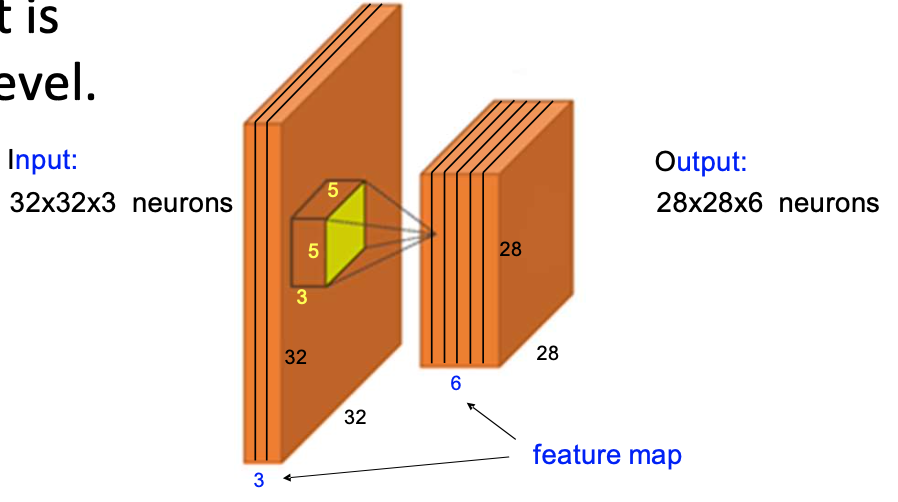
\includegraphics[scale=.5]{images/cnn/weights.png}
    \centering
\end{figure}
\newpage
\paragraph{Un layer tipico di una convolutional network.} Esistono due varianti terminologiche, mostrate nel seguito:
\begin{figure}[!h]
    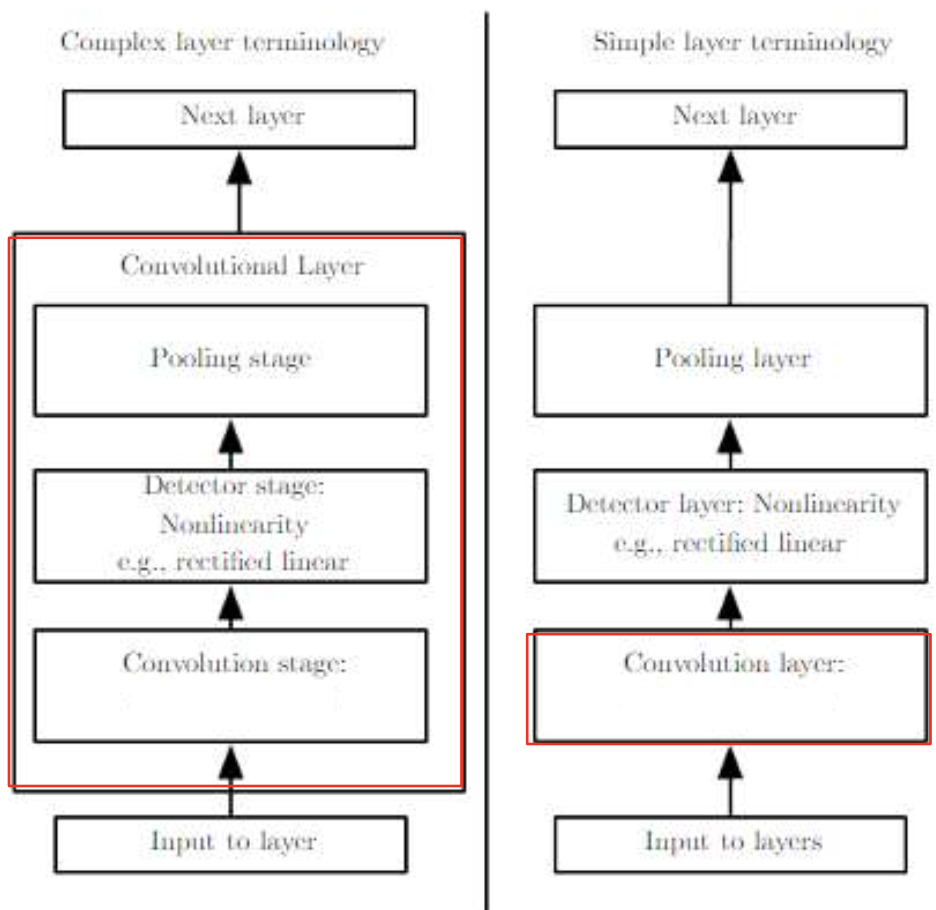
\includegraphics[scale=.4]{images/cnn/typical_layer.png}
    \centering
\end{figure}
\section{Activation function: ReLU}
Storicamente, il multilayer perceptron usa una funzione di attivazione sigmoide. Nelle deep networks però l'uso della sigmoide è problematico a causa dei problemi della back propagation (come il vanishing gradient). Inoltre per valori grandi e piccoli la derivata si avvicina allo $0$.
\begin{figure}[!h]
    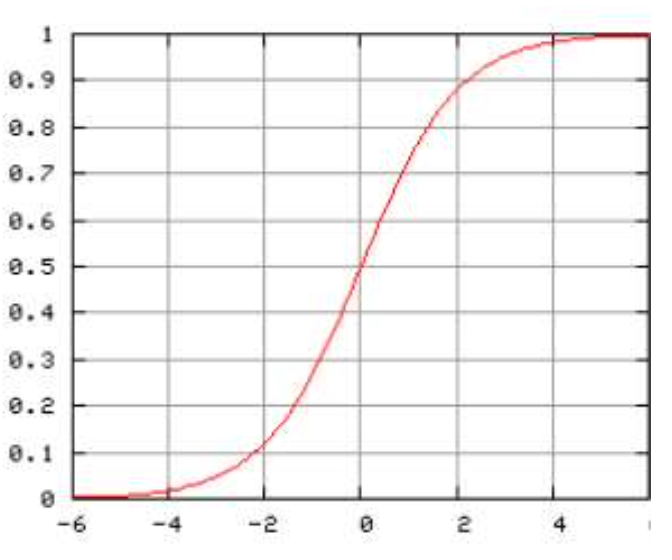
\includegraphics[scale=.4]{images/cnn/sigmoid.png}
    \centering
\end{figure}


La formula per l'aggiornamento dei pesi è:
\begin{equation}
    \delta^l = \big( (\textbf{W}^{l+1})^T \delta^{l+1} \big) \odot \sigma' (a^l).
\end{equation}
Se $\phi$ è vicino a zero, allora il prodotto sarà molto piccolo, portando al vanishing gradient.
\newline
\newline
La risoluzione di questo problema sta nell'utlizzo della \textbf{ReLU (Rectified Linear Unit)} come activation function, che ha derivata $0$ per valori negativi e $1$ per valori positivi:
\begin{figure}[!h]
    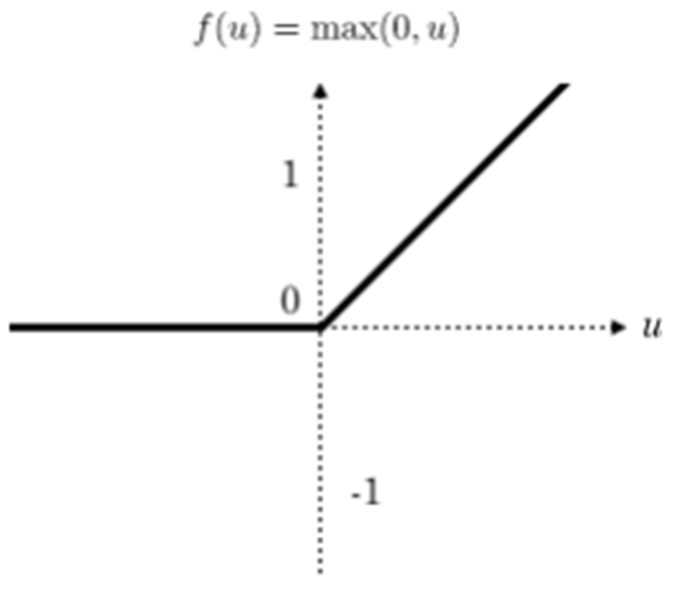
\includegraphics[scale=.4]{images/cnn/relu.png}
    \centering
\end{figure}


Questo conduce alla sparsità delle attivazioni (a causa del fatto che alcuni neuroni sono spenti), e a pattern di attivazione più semplici, quindi più generalizzabili.


Le unità agiscono come \textbf{feature detector} che segnalano quando trovano un match sufficientemente buono per il loro kernel.
\newpage
\section{Pooling layer}
Una \textbf{pooling function} rimpiazza gli output in una certa posizione della rete con con una statistica riassuntiva degli output vicini. Ad esempio, il\textbf{ max pooling operator} riporta l'output maggiore all'interno di un rettangolo.
\begin{figure}[!h]
    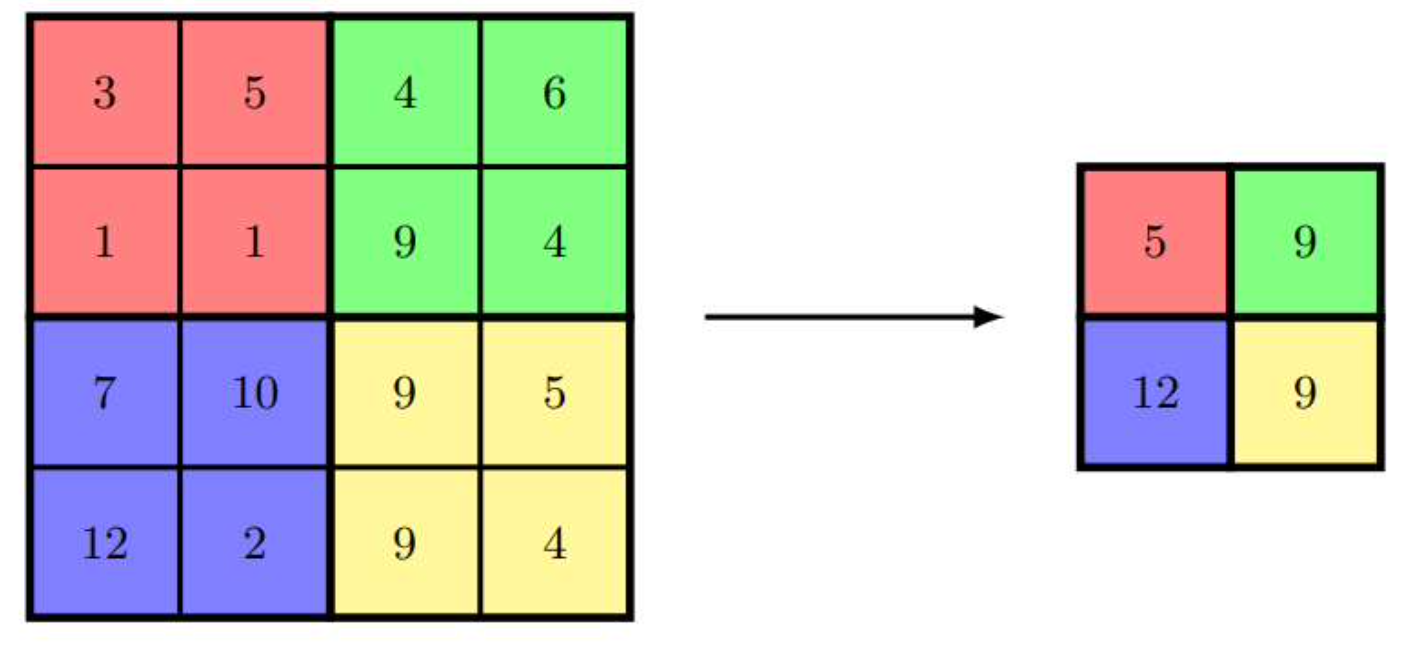
\includegraphics[scale=.4]{images/cnn/pooling.png}
    \centering
\end{figure}
\subsection{Tipologie}
\begin{figure}[!h]
    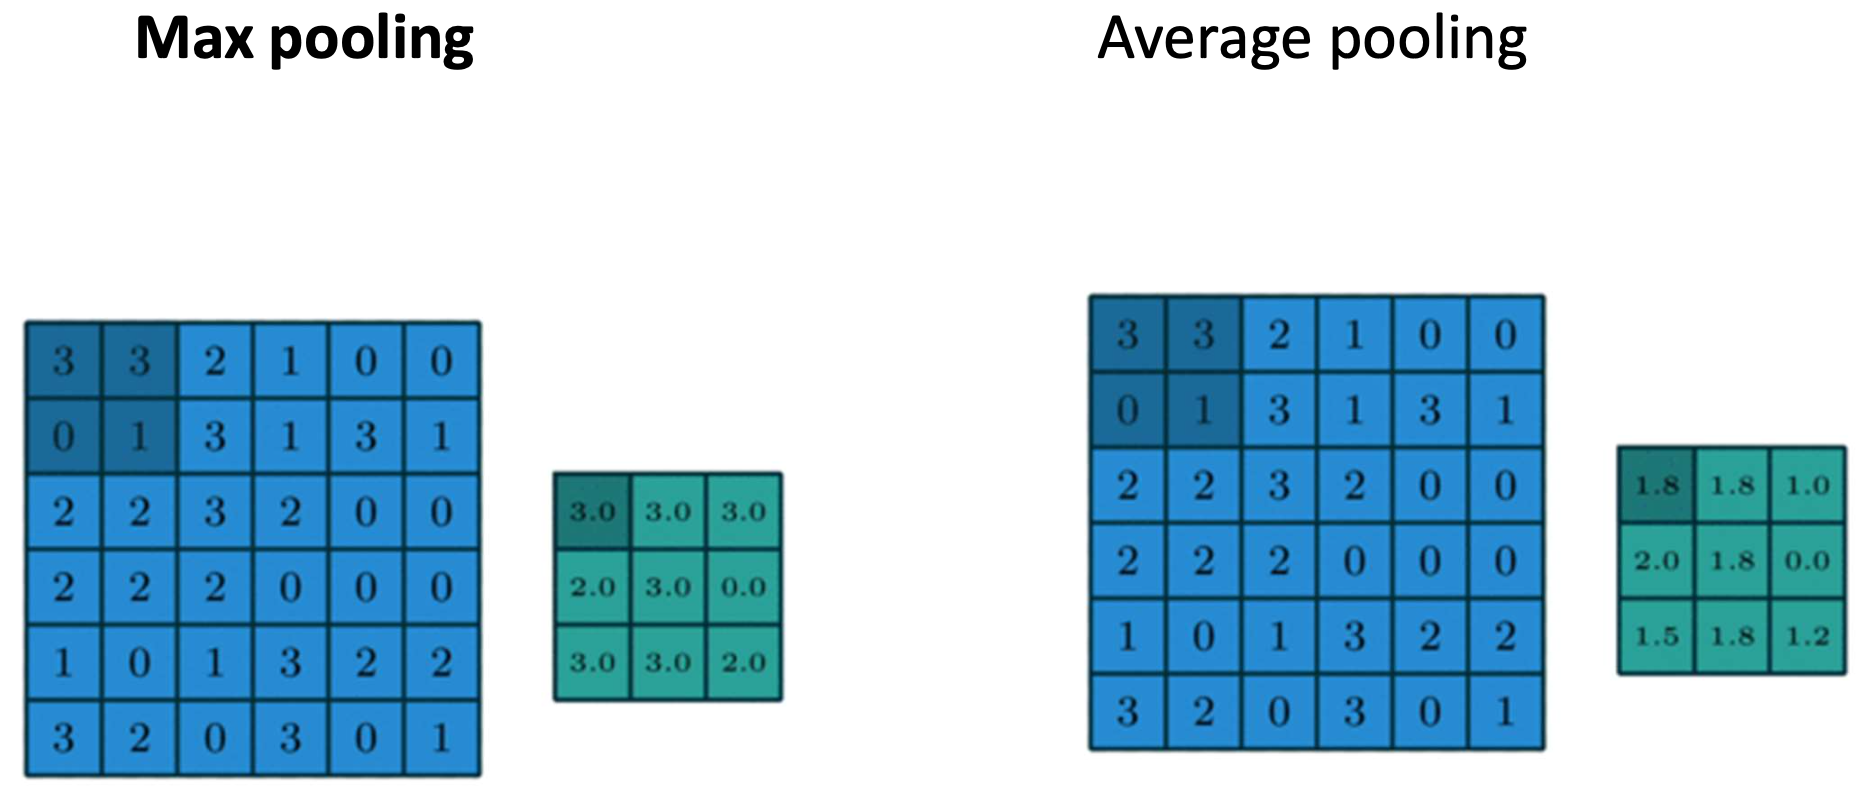
\includegraphics[scale=.4]{images/cnn/types.png}
    \centering
\end{figure}
\subsection{Funzionamento}
Il \textbf{pooling} agisce come \textbf{riduttore della dimensionalità (downsampling)}.
\begin{figure}[!h]
    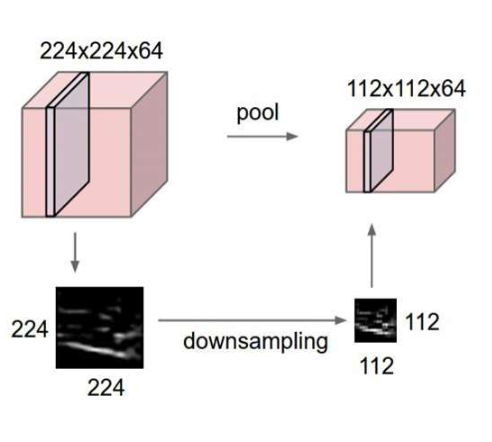
\includegraphics[scale=.6]{images/cnn/pooling_function.png}
    \centering
\end{figure}


Il pooling seleziona i valori \textbf{valori più informativi}. Implementa l'\textbf{invarianza} rispetto a (piccole) traduzioni e i pooling layer \textbf{non hanno pesi}. Il pooling \textbf{non ha parametri apprendibili ma solo iperparametri} (fissati dall'architettura): una scelta standard è il max pooling su kernel $2\times2$ con passo $2$.
In generale, \textbf{è applicato alle regioni non sovrapposte}.
Il pooling viene solitamente applicato a ciascun canale di una feature map in modo indipendente.
Meno frequentemente può essere applicato su più canali di feature map.
\newpage
Le CNNs \textbf{contengono multipli strati di layer convoluzionali e di pooling in successione}, nei quali i canali di output di un particolare layer formano i canali di input del layer successivo (analogamente ai canali RGB del livello di input). Uno o più blocchi convoluzionali estraggono feature di livello progressivamente più elevato.


Un esempio di struttura è il seguente:
\begin{figure}[!h]
    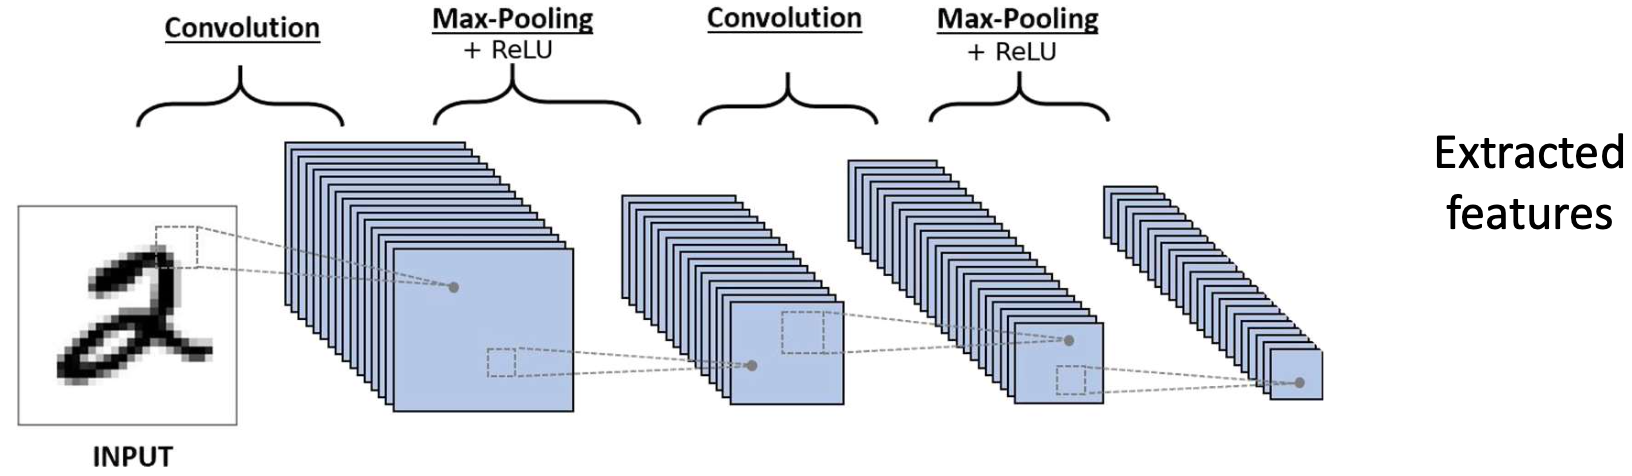
\includegraphics[scale=.5]{images/cnn/ex01.png}
    \centering
\end{figure}


Per esempio, se il livello precedente ha $n$ canali, ogni filtro avrà $n$ canali (se le feature maps di un precedente convolutional layer sono $6$, i filtri del livello successivo avranno dimensione $5\times5\times6$).
\newline
\newline
\textbf{Nella parte finale della rete è presente uno (o più)  fully connected layer il cui input è l'output del max pooling layer precedente, "flattened"}. In quest'ultimo layer c'è un neurone per ogni categoria di output, è quindi effettivamente questo il momento in cui si assegna l'etichetta. Di solito, per determinare il valore di output, viene utilizzata una \textbf{soft max function}.
\begin{figure}[!h]
    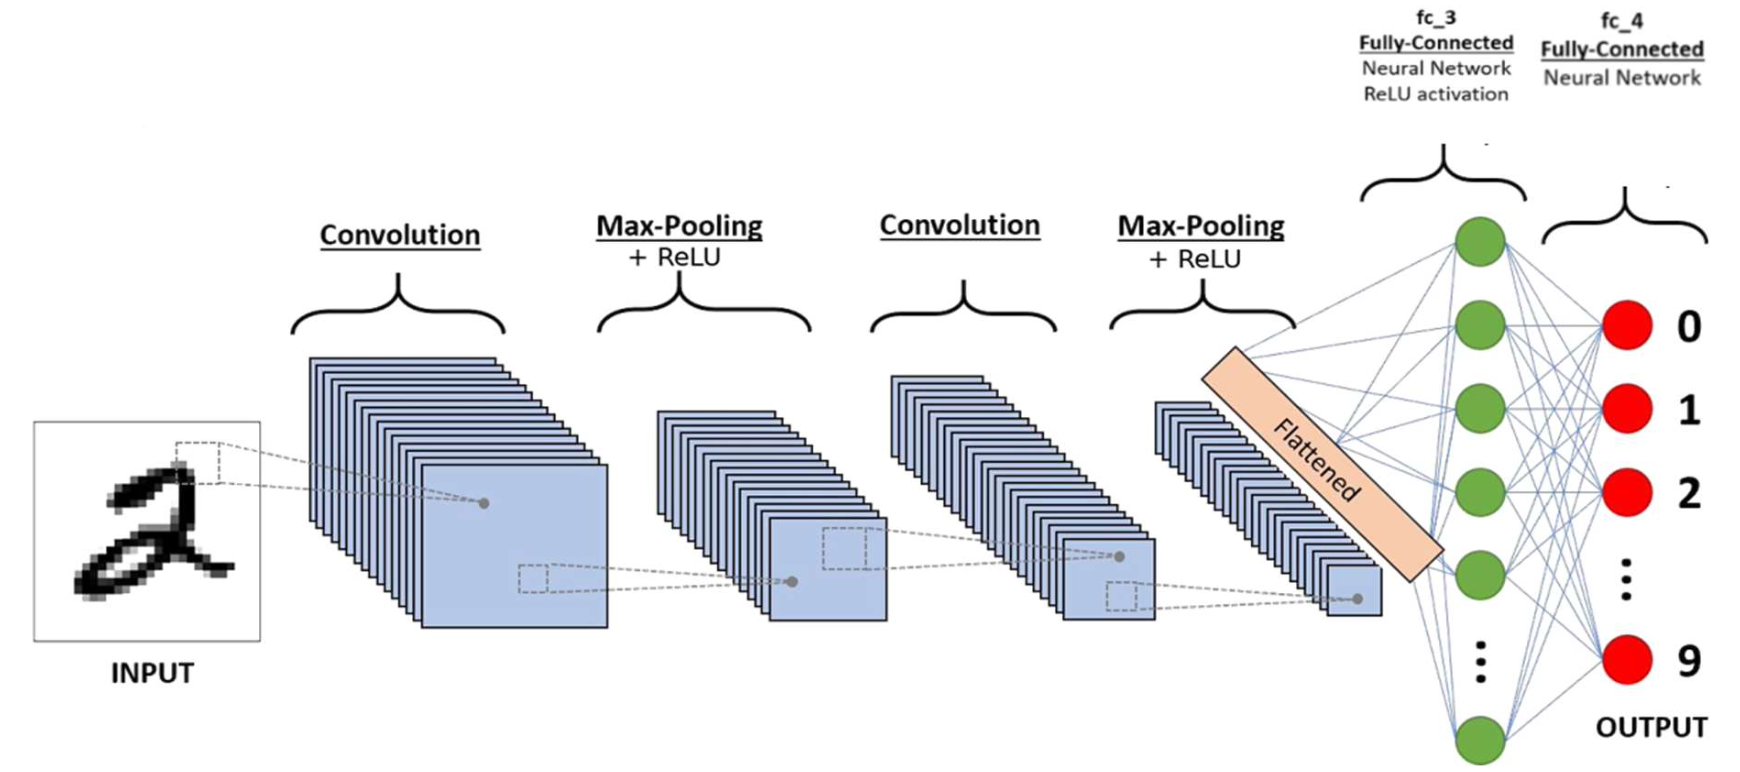
\includegraphics[scale=.5]{images/cnn/last_layer.png}
    \centering
\end{figure}
\newpage
\section{Cost function}
L'idea che il valore che porterà la scelta dell'output \textbf{può essere visto come probabilità}. Nel campo delle cost function, quando vengono trattati classificatori, alcune scelte comuni sono:
\begin{itemize}
    \item l'utilizzo di una \textbf{SoftMax function} nel final layer. Consiste in $s$ neuroni (uno per ogni classe) \textbf{fully-connected ai neuroni del layer precedente}. Gli input $v_k$ dei neuroni vengonocì calcolati come al solito, ma come funzione di attivazione del $k-$esimo neurone utilizziamo
    \begin{equation}
        z_k=f(v_k)=\frac{e^{v_k}}{\sum_{c=1,\dots,s}e^{v_c}},
    \end{equation}
    dove i valori $z_k$ possono essere visti come \textbf{probabilità}: possono assumere i valori $[0,\dots,1]$ e la loro somma è pari ad $1$;
    \item utilizzo della \textbf{multi-class Cross-Entropy come loss function} (in sostituzione della mean squared error, introdotta per il multilayer perceptron). La cross-entropy \textbf{misura quanto la  predetta distribuzione $p$ differisce dall'output desiderato}.
    \begin{equation}
        \text{Cross-Entropy Loss}=-\sum^s_{i=1}y_i\cdot\log{(p_i)},
    \end{equation}
    dove $y_i$ è l'output desiderato per l'$i-$esimo neurone e $p_i$ è invece il valore predetto.
\end{itemize}

\textbf{In questo caso, l'algoritmo di learning utilizzato è la backpropagation e l'idea è che questa volta utilizziamo la cross entropy come loss function}. Essa restituisce un valore alto quando il valore predetto per una data categoria è diverso da quello aspettato, diversamento restituisce un valore basso. La cross-entropy tra due distribuzioni discrete $p$ e $q$ misura, come detto, quanto $p$ differrisce da $q$ ed è definita come:
\begin{equation}
    H(p,q) = -\sum_vp(v)\dot\log{(q(v))}.
\end{equation}

A questo punto sono presenti tutti gli ingredienti e siamo pronti per cominciare l'apprendimento. Il dataset viene splittato in tre parti:
\begin{itemize}
    \item \textbf{training set};
    \item \textbf{validation set};
    \item \textbf{test set}.
\end{itemize}
La rete viene \textit{trainata} sul \textbf{training set} per qualche epoca, a quel punto si vede come si comportano i pesi sul \textbf{validation set}. Questo passaggio è fatto per diversi motivi, su tutti abbiamo il fatto di monitorare l''aprendimento, \textbf{apprendere gli iperparametri} ed eventualmente fermare l'apprendimento se ci si accorge che si sta andando in contro ad \textbf{overfitting}. Infine, il \textbf{test set} è utlizzato per testare la \textbf{capacità di generalizzare} della rete.


Tipiche proporzioni dei tre sottoinsiemi sono:
\begin{itemize}
    \item training set: da $70\%$ a $80\%$;
    \item validation set: da $10\%$ a $15\%$;
    \item training set: da $10\%$ a $15\%$.
\end{itemize}

\newpage
\paragraph{ImageNet.} Il dataset più conosciuto ed utilizzato per questo tipo di reti è \textbf{ImageNet}. Si tratta di un dataset di milioni di immagini naturali etichettate in $22000$ categorie. L'introduzione di dataset enormi, come ImageNet, ha permesso ed accelerato lo sviluppo di reti convoluzionali. Alcune delle immagini di ImageNet: 
\begin{figure}[!h]
    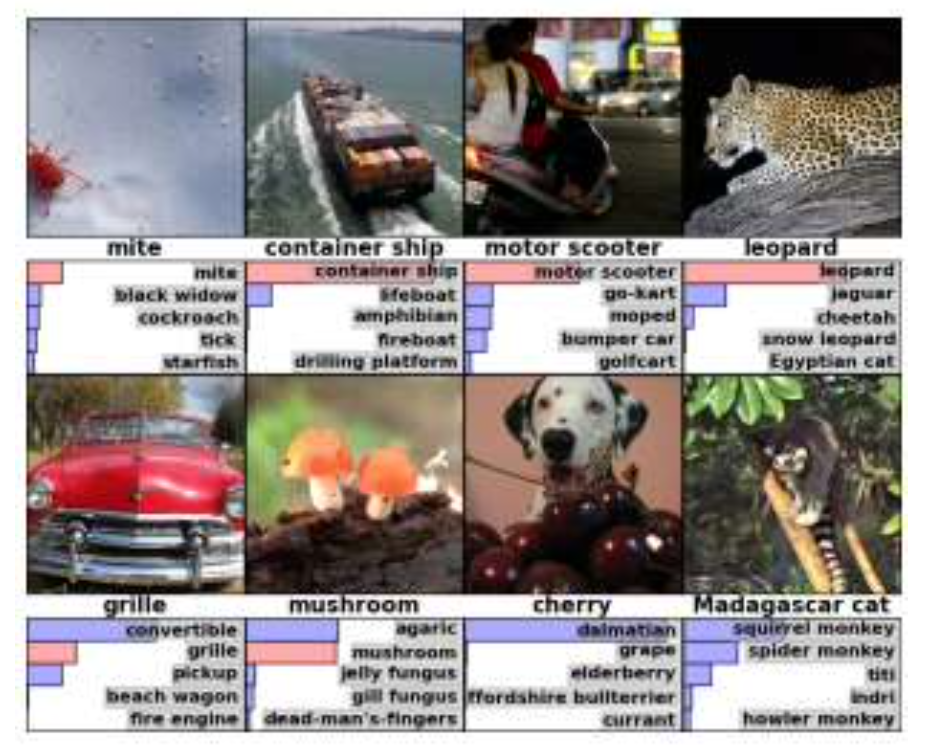
\includegraphics[scale=.5]{images/cnn/imagenet.png}
    \centering
\end{figure}


La \textbf{ImageNet Large Scale Visual Recognition Challenge (ILSVRC)} è una competizione in cui si valutano algoritmi per il rilevamento di oggetti e la classificazione di immagini su larga scala.
\begin{figure}[!h]
    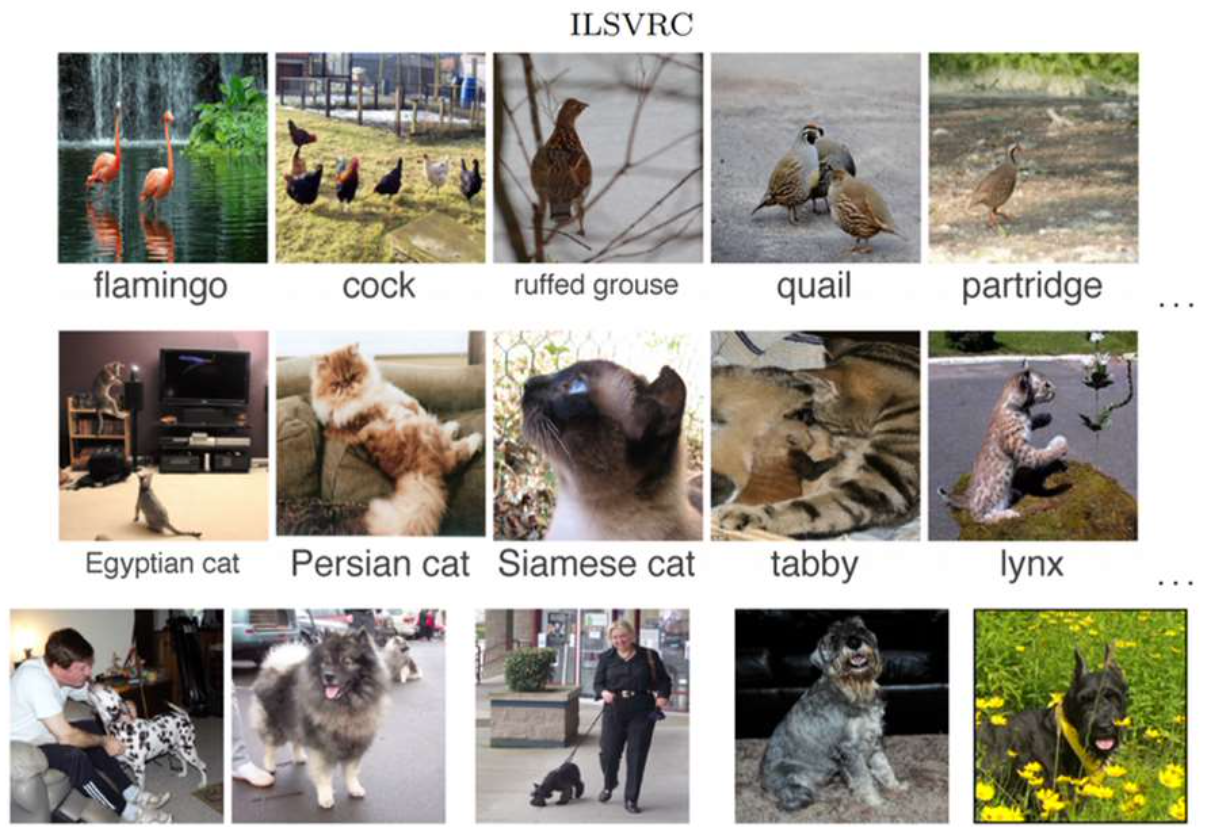
\includegraphics[scale=.5]{images/cnn/ilsvrc.png}
    \centering
\end{figure}
Vedremo degli esempi di architetture che mixano in modo diverso i vari ingredientri che abbiamo introdott e tutte fanno visual recognition. \textbf{AlexNet} è stata la prima cnn che a vincere la competizoine nel 2012. Da quel momento in poi, di anno in anno, vengono sviluppate CNNs sempre più potenti e performanti, anche grazie alla veloce e continua evoluzione di modelli.
\newpage
\section{Evitare l'overfitting}
Finora abbiamo dato un'idea generale di come le CNNs sono fatte e lavorano (architetture, loss function, ecc). Esistono però delle tecniche che usiamo per prevenire l'overfitting e migliorare le performance. Una è stata introdotta proprio da AlexNet, la \textbf{dropout generalization}:


l'idea è che \textbf{durante l'apprendimento, spegniamo (dropout) randomicamente alcuni neuroni}, scelti con probabilità $p$. I grossi vantaggi di pratica sono:
\begin{itemize}
    \item accelerare il processo di training;
    \item incoraggiare lo sviluppo di \textbf{rappresentazione sparsa}, che significa generalizzare meglio ed evitare overfitting.
\end{itemize}
\begin{figure}[!h]
    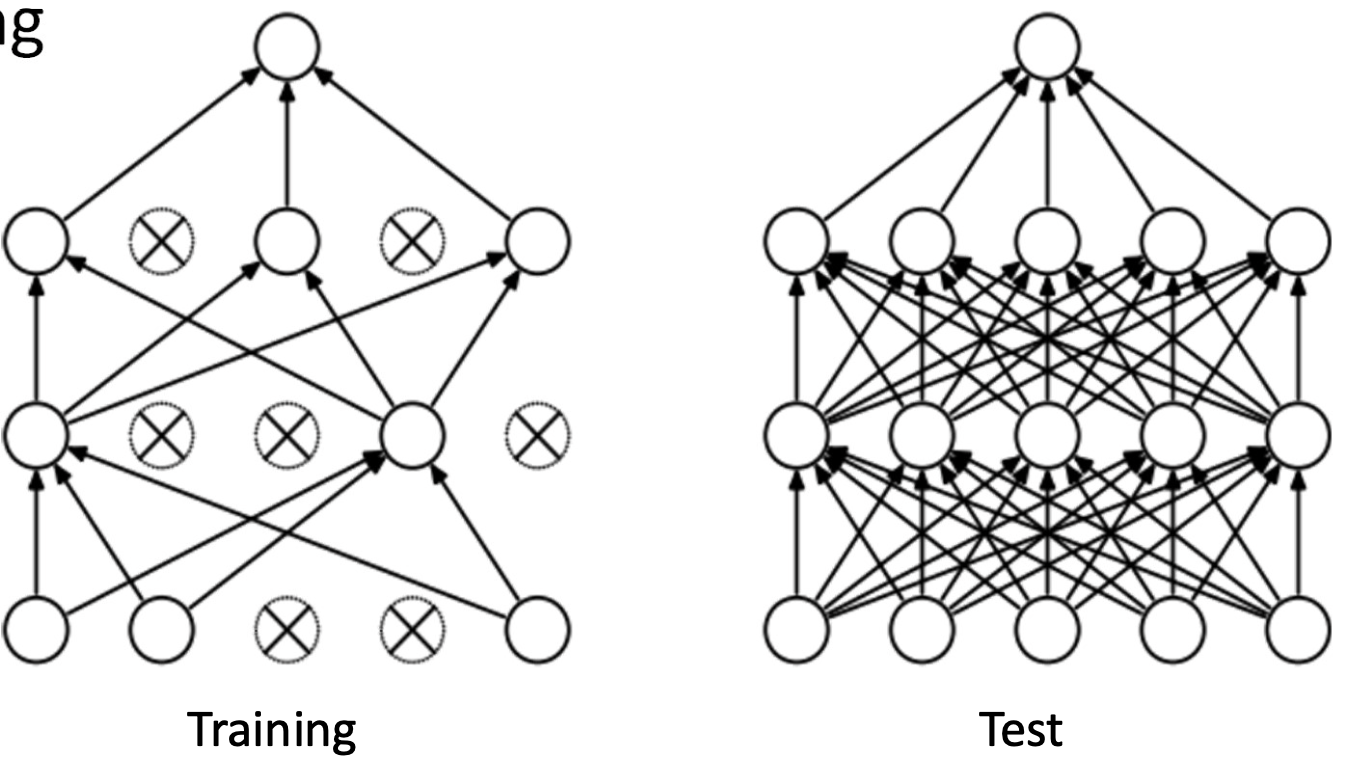
\includegraphics[scale=.5]{images/cnn/dropout.png}
    \centering
\end{figure}
L'idea è che la rete non possa contare su tutti i neuroni, quindi l'obiettivo è usarne meno ed essere più generali possibili.

\paragraph{Early Stopping.} Vengono monitorate le performance del modello sul validation set durante l'apprendimento ed \textbf{il processo viene bloccato quando esse cominciano a degradare} (infatti ciò indica overfitting). E' sostanzialmente un mondo per non permettere al modello di contuare ad imparare rumoere presente nei data di training, dopo il punto ottimale.

\paragraph{Data Augmentation.} \textbf{(**Saltato a lezione**)} Not a regularization technique in the traditional sense. It artificially increases the size of the training dataset by applying random transformations (like rotation, flipping, scaling) to the training images.
This helps the model generalize better by exposing it to variations it might encounter in real-world scenarios.

\paragraph{Batch Normalization.} \textbf{(**Saltato a lezione**)} It normalizes the output of each layer, which can reduce overfitting by introducing noise to the training process.

\paragraph{Weight Decay.} Viene aggiunta una \textbf{penalità alla loss function} che incoraggia pesi piccoli, prevenendo l'overfitting.
\newpage
\section{Esempi di CNNs}
La prima cnn fu \textbf{LeNet}, introdotta negli anni 80. Era usata per classificare semplici cifre scritte a mano.
\begin{figure}[!h]
    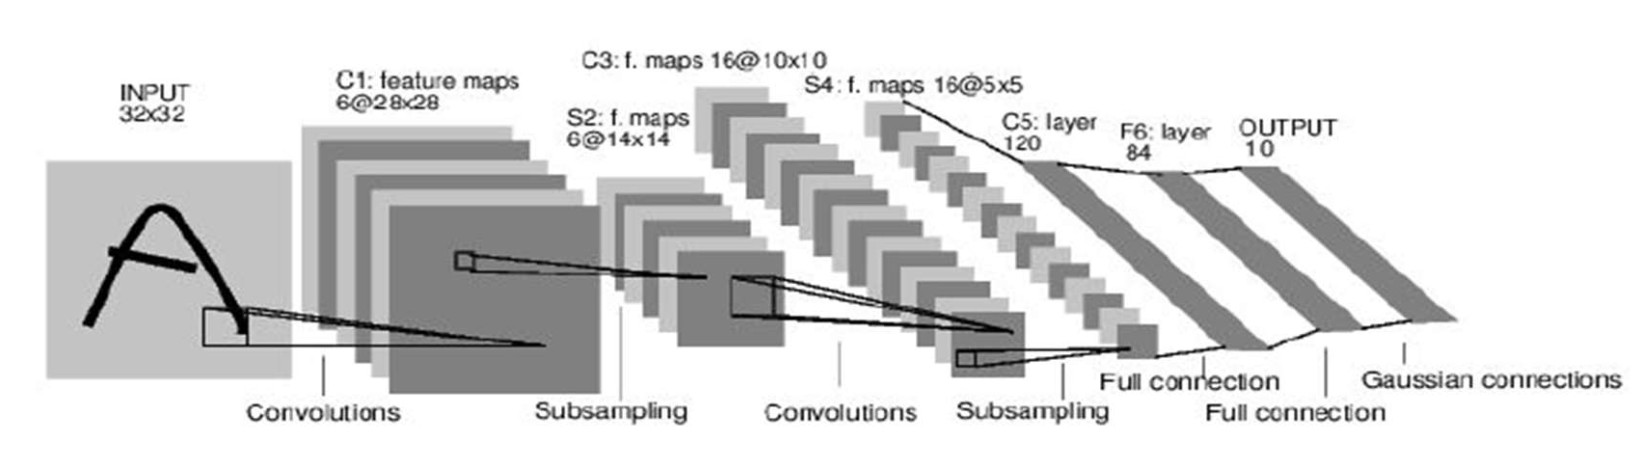
\includegraphics[scale=.5]{images/cnn/lenet.png}
    \centering
\end{figure}



Venne poi il turno di \textbf{AlexNet}, che determinò il burst di questa architettura. Vinse la competizione di ImageNet nel 2012 con il risultato del $15\%$ di error rate nelle top 5 categorie.
\begin{figure}[!h]
    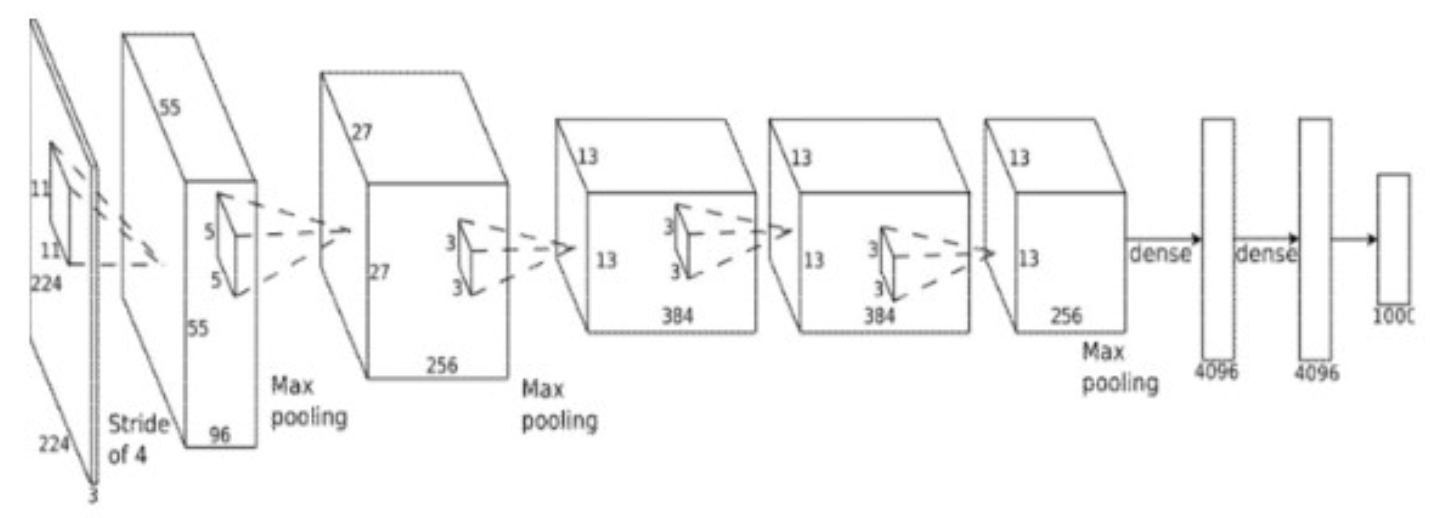
\includegraphics[scale=.5]{images/cnn/alexnet_ex.png}
    \centering
\end{figure}



Questo è stato il punto di partenza dell'evoluzione delle CNNs, da qui in poi abbiamo avuto più o meno sempre gli stessi elementi fondazionali ma diversi iperparametri.
\newline
\newline
\textbf{VGG-16 Modeli} è dotata di 16 livelli e ha un modo fissato di di specificare gli iperparametri. Per esempio tiene fissati tutti i kernel.
\begin{figure}[!h]
    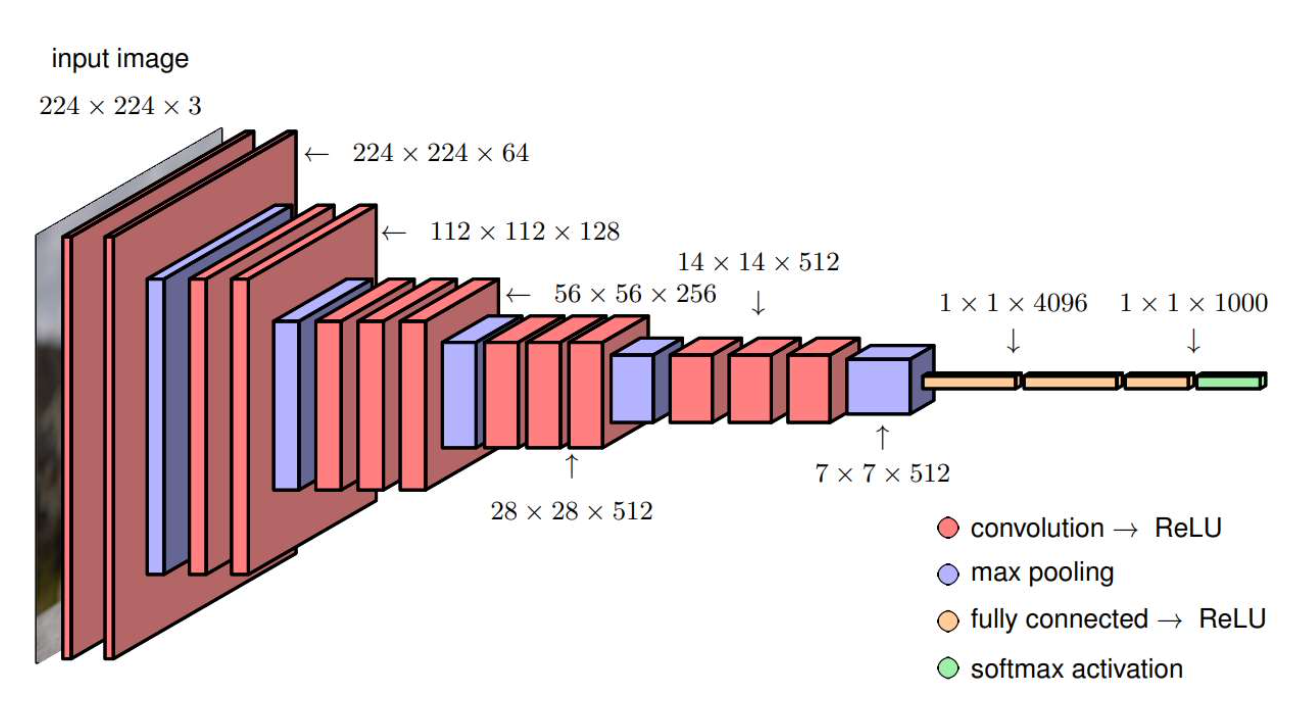
\includegraphics[scale=.5]{images/cnn/vgg.png}
    \centering
\end{figure}
\newpage
Oggi abbiamo la \textbf{ResNet family}, di cui  non andiamo nei dettagli in quanto abbiamo sempre le solite combinazioni. Le reti di questa famiglia possono essere molto profonde, grazie a dei link che permettono di saltare alcuni layer. 
\begin{figure}[!h]
    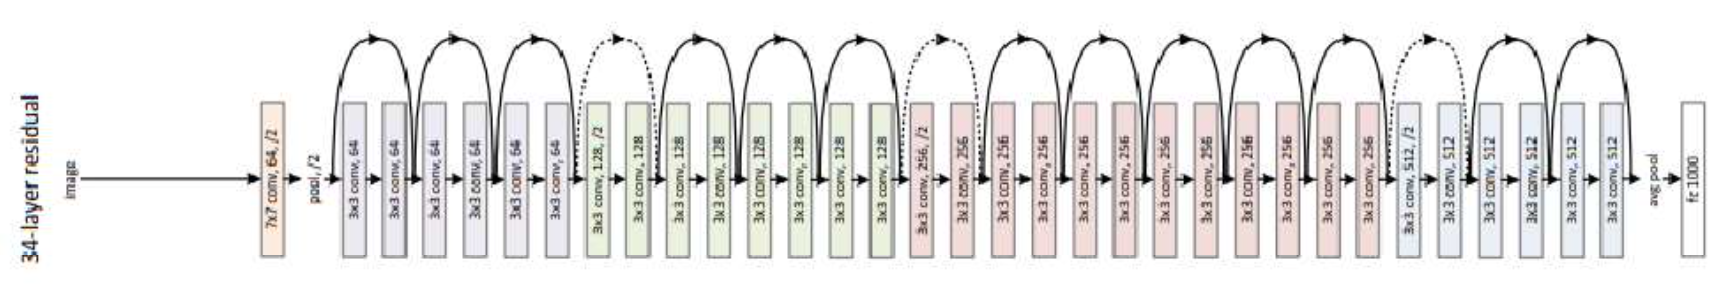
\includegraphics[scale=.5]{images/cnn/resnet.png}
    \centering
\end{figure}


L'ultimo esempio di architettura che vediamo è quello della \textbf{Inception Family}. In questo caso ogni livello è una combinazioni di diverse scelte di iperparamtri. La prima rete di questa famiglia era stata chiamata era \textbf{GoogLeNet} come omaggio a LeNet (sono seguite poi \textbf{V2}, \textbf{V3}, ecc).
\begin{figure}[!h]
    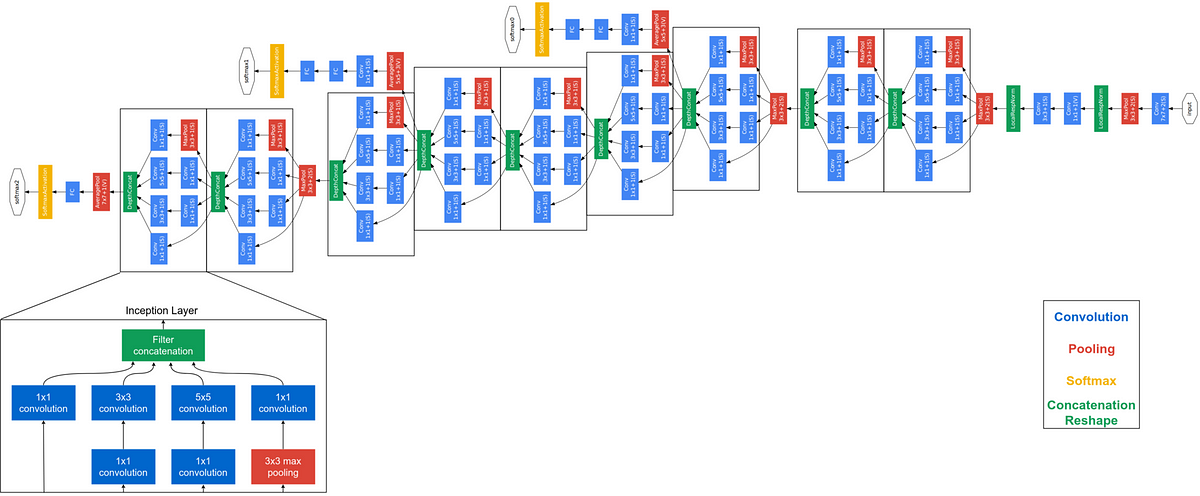
\includegraphics[scale=.35]{images/cnn/inception.png}
    \centering
\end{figure}
\newpage
\section{Transfer Learning}
Il problema principale delle CNNs è il fatto che \textbf{abbiano perfomance molto buone quando applicate a dataset molto grandi}, (come ImageNet) diversamente non si comportano così bene. A causa del fatto che non sempre si hanno a disposizione dataset così grandi, viene normalmente utilizzato il \textbf{transfer learning}. L'idea è che possiamo applicare la nostra rete, inizialmente utilizzata su un problema, ad un secondo problema (della stessa tipologia primo ma con dati diversi). I passi sono i seguenti:
\begin{itemize}
    \item cominciamo con una rete pre-trained, appresa su un problema simile al secondo su cui verrà applicata;
    \item rimpiazziamo il layer di output con un nuovo layer di neuroni softmax (eventualmente adattati al numero di classi del secondo problema);
    \item come valori iniziali dei pesi usiamo quelli della rete pre-trained, ad eccezione delle connession tra il penultimo e l'ultimo layer, i quali pesi sono inizializzati in maniera casuale;
    \item eseguiamo le nuove iterazioni dper ottimizzare ipesi rispetto alle peculiarità del nuovo dataset (non è necessario che sia di grandi dimensioni).
\end{itemize}
\begin{figure}[!h]
    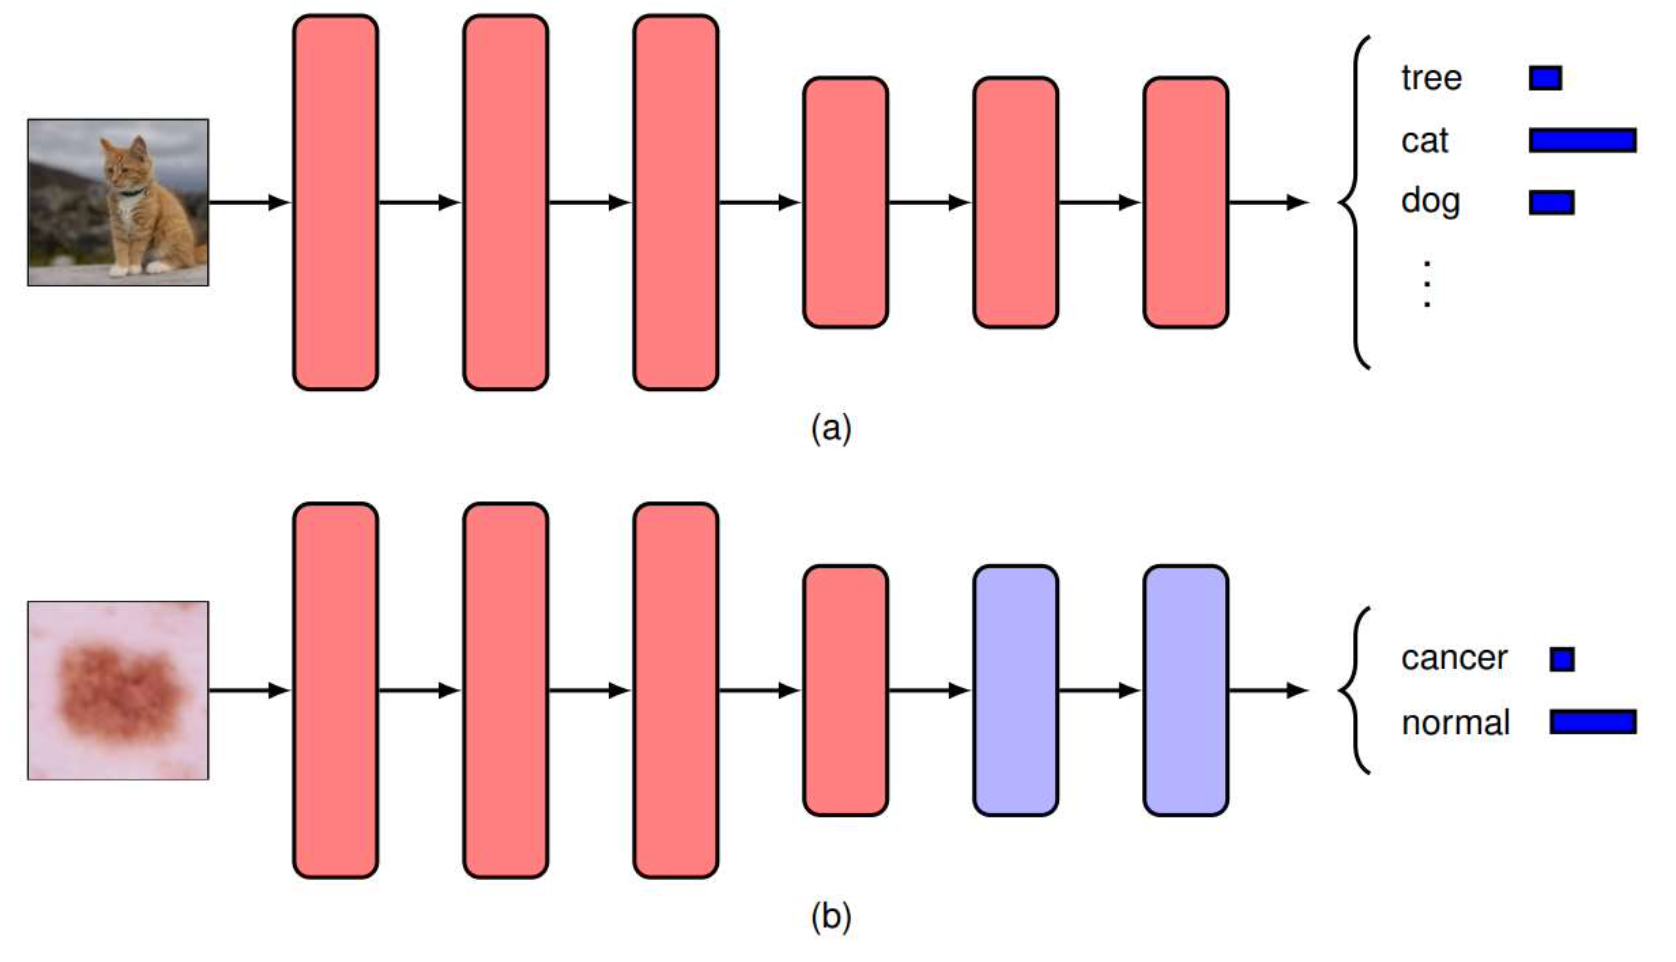
\includegraphics[scale=.5]{images/cnn/transf_learning.png}
    \caption{La rete è stata prima applicata ad un problema di classificazione di gatti e poi di cellule cancerogene. I layer della rete originale sono indicati in rosso, i nuovi layer in blu.}
    \centering
\end{figure}


E' stato dimostrato che questo tipo di approccio fornisce risultati buoni.
\newline
\newline
\textbf{Esistono delle varianti del transfer learning}, una delle quali funziona sostanzialmente come la variante principale ad eccezione del fatto che classificatore esterno è utilizzato per classificare i patter appartenenti al nuovo dominio.
\newpage
\section{Altri task}
\paragraph{Object Detection.} Le CNNs possono ovviamente essere applicate anche ad altri task oltre la classificazione. Uno di questo è la cosiddetta \textbf{object detection}: in questo caso solo gli oggetti all'interno di un'immagine non vengono solo classificati, ma anche \textbf{localizzati}. Per riuscire a risolvere questo tipo di task le CNNs devono essere \textbf{adattate}.
\begin{figure}[!h]
    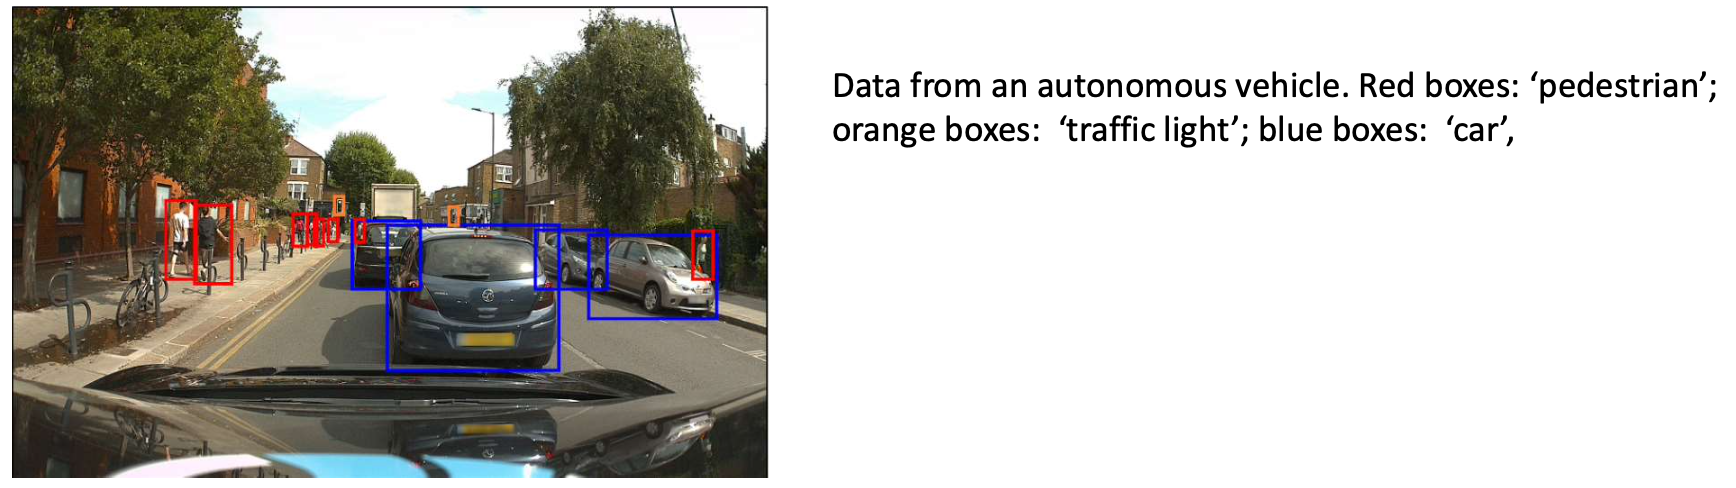
\includegraphics[scale=.5]{images/cnn/obj_det.png}
    \centering
\end{figure}



\paragraph{Image Segmentation.} Un altro tipo di task a cui le CNNs possono essere adattate è la \textbf{image segmentation}. Qui possono essere usate per \textbf{identificare tutti i pixel dell'immagine che corrispondono a date categorie}. Ogni pixel viene classificato individualmente dividendo l'immagine in regioni che condividono un'etichetta comune. 
\begin{figure}[!h]
    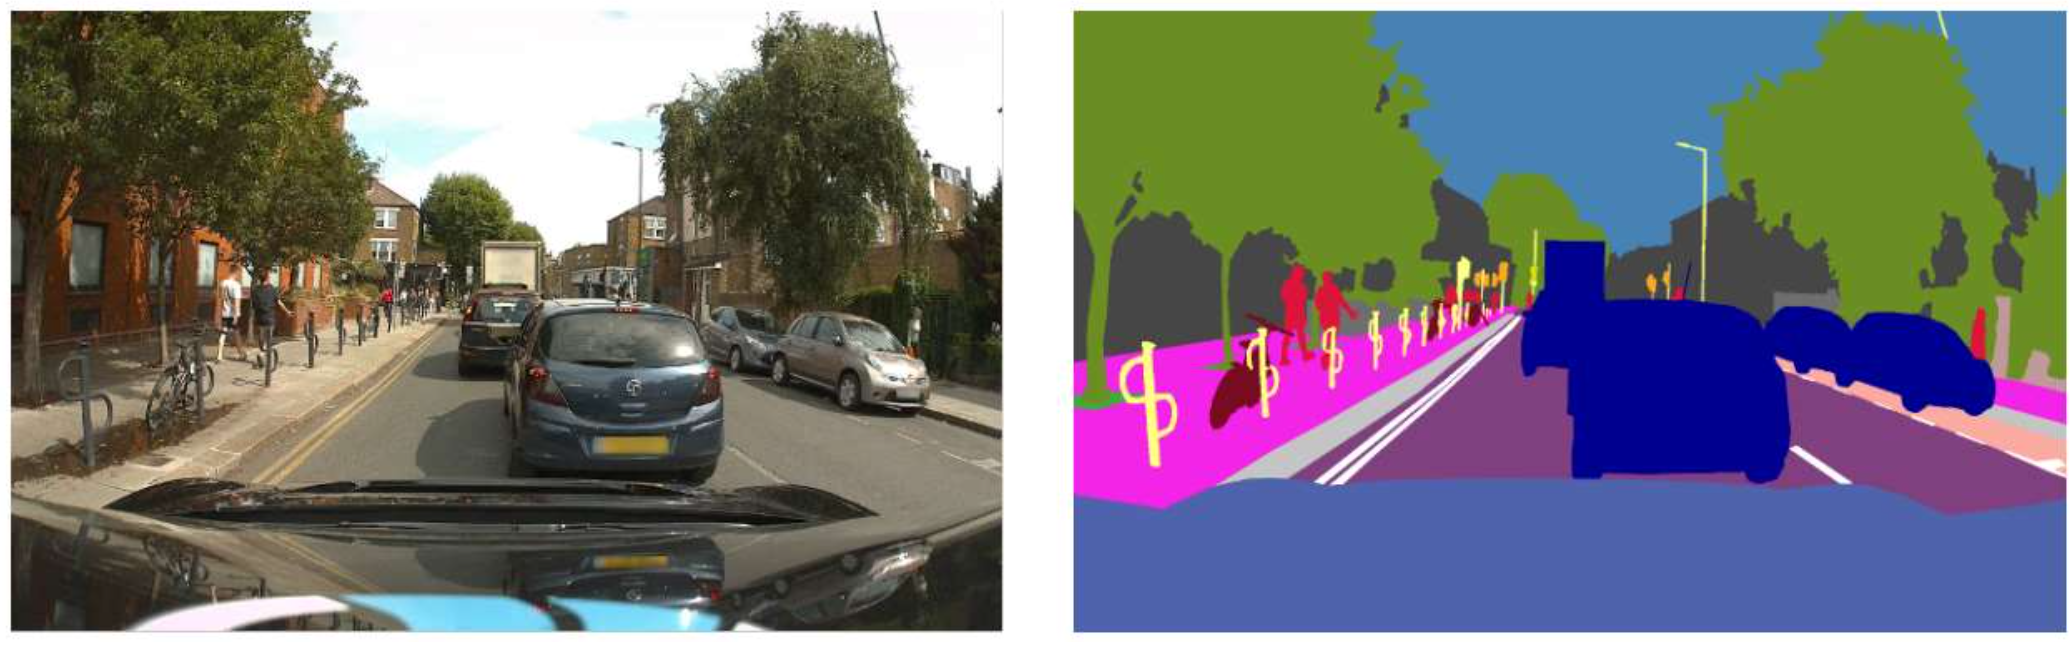
\includegraphics[scale=.45]{images/cnn/img_segm.png}
    \caption{pixel blu “macchina”; pixel rossi “pedonale”; pixel arancioni “semaforo”}
    \centering
\end{figure}



Ci sono diversi modi per adattare CNNs che sono state orignariamente pensate per risolvere task di classificazione, alla risoluzione di altri task. Uno di questi, per l'adattamento a object detection o localization, è \textbf{Fast R-CNN}: l'immagine in input viene scannerizzata e la rete prova a riconoscere porzioni di imaggini che \textbf{crede con alta probablità} far parte di una categoria.
\begin{figure}[!h]
    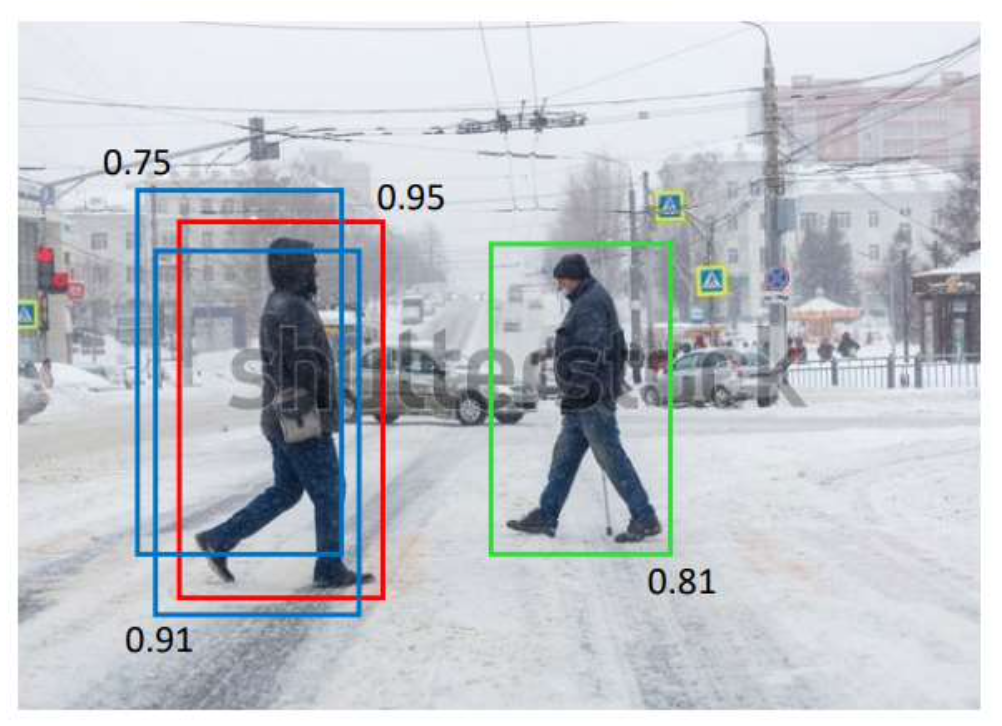
\includegraphics[scale=.45]{images/cnn/rcnn.png}
    \centering
\end{figure}

\newpage



\section{Un po' di storia}
Come precedentemente detto,  \textbf{le CNN estraggono feature da immagini, le quali feature vanno complicandosi man mano che si procede al loro riconoscimento}. Queste reti essenzialmente \textbf{riproducono alcuni pattern che usiamo nel nostro cervello}: è stata infatti scoperta a partire da un esperimento su gatti, \textbf{l'esistenza di semplici neuroni che hanno il compito di rilevare feature semplici}. Seguono poi altre cellule, più complesse, che \textbf{combinano le informazioni e che sono sensibili a feature più complesse}. 


Molti ricercatori hanno cercato di capire se il parallelismo tra CNNs e cervello umano (o animale in questo caso) fosse consistente o no, ma quello che è sicuro è che questa sia stata una delle motivazioni fondamentali alla base dell'utilizzo di CNNs.
\begin{figure}[!h]
    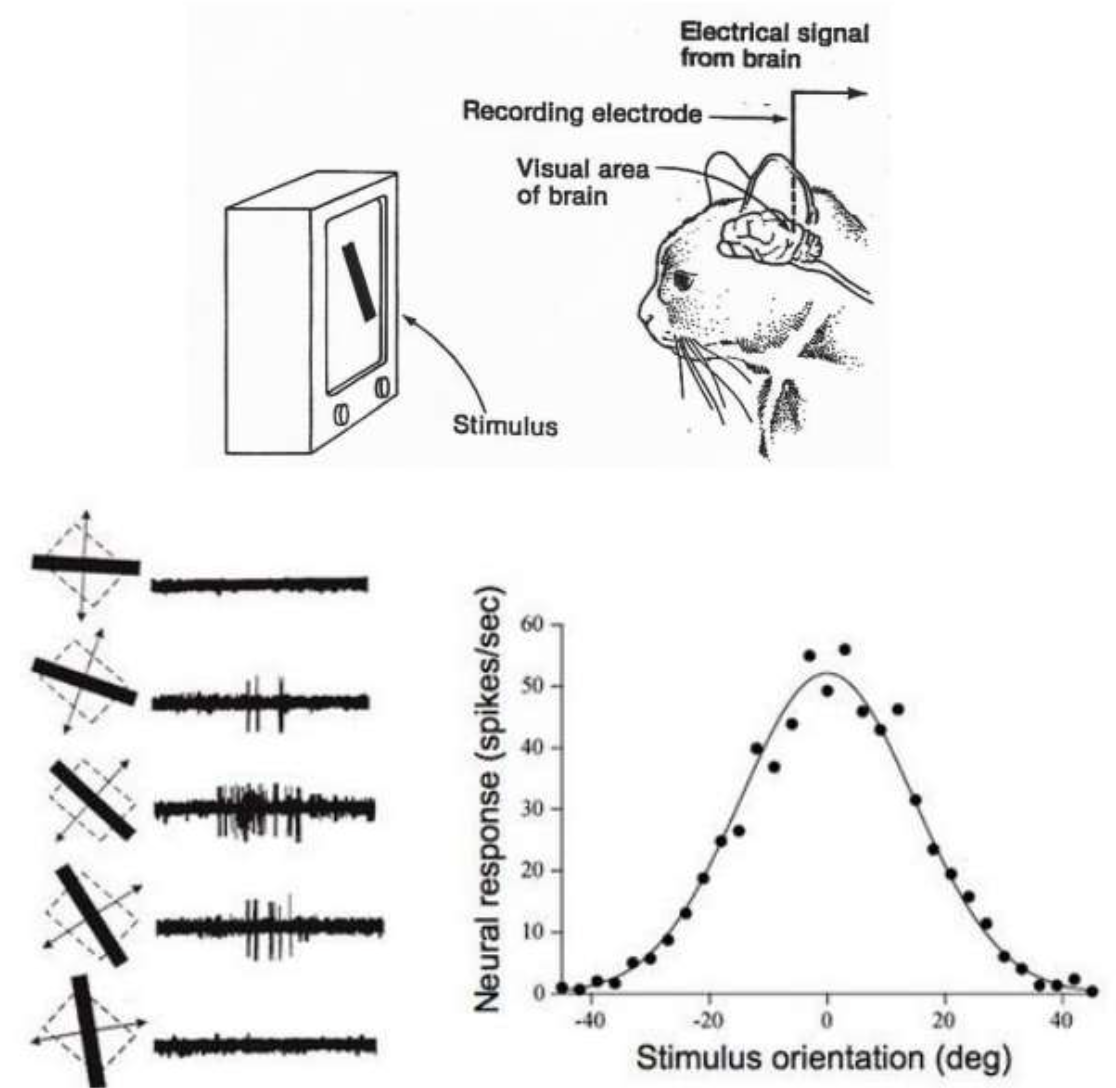
\includegraphics[scale=.45]{images/cnn/cat_brain.png}
    \centering
\end{figure}


L'immagine seguente prova a specificare ciò che è stato appena detto. 
Viene esplicitato quello che è il parallelismo tra il processo nella CNN 
(sotto) e quello nel cervello (sopra). Su YouTube è presente un video 
sull'esperimento di Hubel e Wiesel, i ricercatori che per primi hanno fatto queste scoperte.
\begin{figure}[!h]
    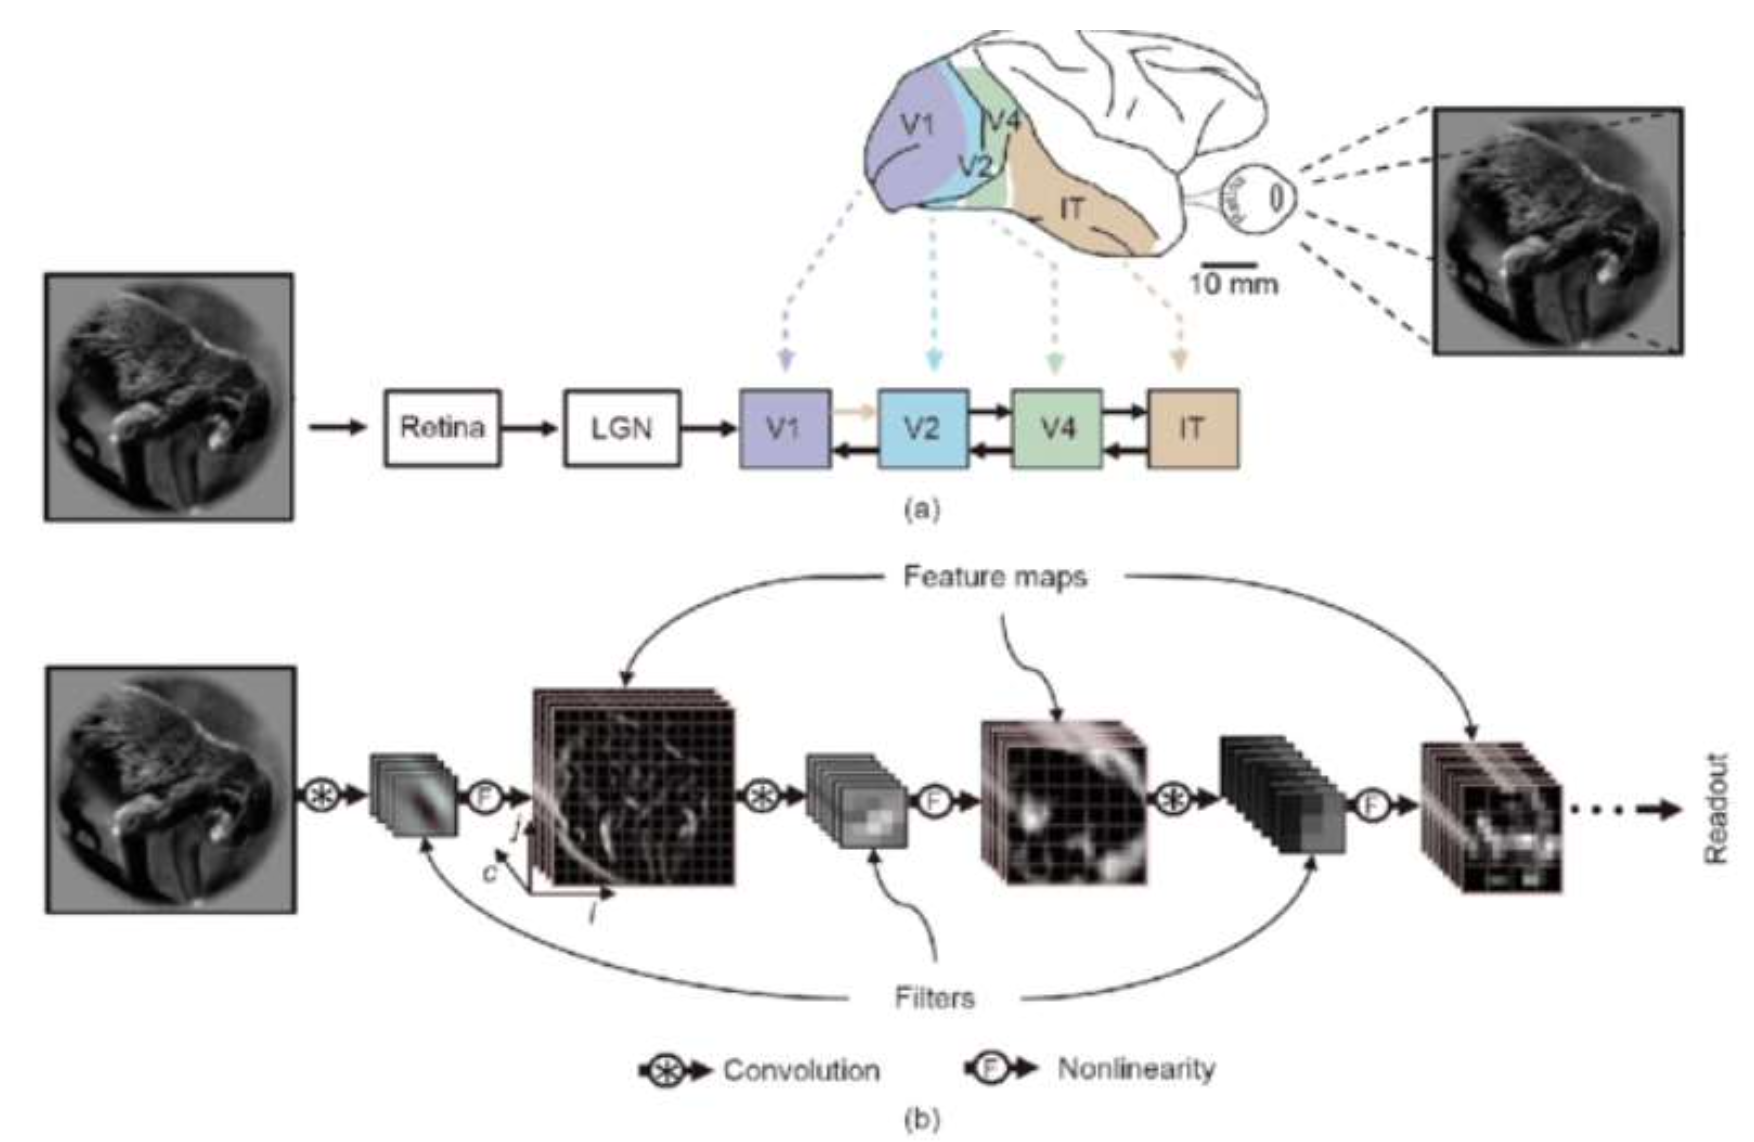
\includegraphics[scale=.35]{images/cnn/exp.png}
    \centering
\end{figure}
\newpage